\chapter{多类生物标记物定位问题的实验评估}\label{sec:multi_classes}
\section{前言}
在上一章中,与包括CAM和Grad-CAM在内的两种可视化方法相比,本文介绍了我们提出的模型在处理二类生物标记物定位问题的优异表现。与上一章内容安排一样,在本章中,我们将本文提出的模型由二类问题推广到多类问题,并展示相关实验结果与分析。首先在\ref{sec:mul_classes_ds_intro}小节中,本文将会介绍实验数据集的相关信息。在\ref{sec:multi_classes_experiment_setting}小节中,本文将会说明实验相关设置,包括学习率、实验超参数、优化器等信息。从\ref{sec:multi_classes_experiments_res}小节开始,本文将展示本文提出的模型在处理多类生物标记物定位问题上的相关实验结果,同样包括与CAM和Grad-CAM的相关对比实验和与判别器网络结构相关的消融实验,随后本文会在\ref{sec:multi_classes_hyper_paras}小节中对超参数组合进行相关测试。注意,由于本章实验相关评价标准与上一章完全一样,所以本章不再作相关赘述。下面展开本章内容的具体阐述。
\section{数据集介绍}\label{sec:mul_classes_ds_intro}
\subsection{多类模拟皮肤病病变数据集}
多类模拟皮肤病病变数据集同样是包含带有人工生物标记物的皮肤图像,图像尺寸大小均为$128\times 128$,图像均以PNG格式存储,每张图像不仅有图像级标注,还有像素级标注,故可用于定量分析有关的实验评估。在\ref{subsec:bin_simulated_skin_ds}小节中用到的二类模拟皮肤病病变数据集基础上额外增加了两类,故多类模拟皮肤病病变数据集中一共有$4$类,其中$3$类异常,$1$类正常。正常类图像是从ISIC2018~\cite{codella2019skin, tschandl2018ham10000}分类任务中的图像\footnote{https://challenge2018.isic-archive.com/task3/}通过滑动窗口方式收集$922$张正常皮肤图像(实际上是图像块)。第一类异常与二类模拟皮肤病病变数据集中的异常类一样,生成过程也相同(相关介绍参见\ref{subsec:bin_simulated_skin_ds}小节)。第二类异常图像中的生物标记物是黑色素瘤病变区域,为了生成这个数据集,我们首先从ISIC2018的分类任务(注意没有重复使用图像)提取了图像大小为$128\times 128$的正常图像(同样通过滑动窗口方式)。同时,我们根据ISIC2018的分割任务\footnote{https://challenge2018.isic-archive.com/task1/}中的黑素瘤区域的像素级标签,将其中的黑素瘤像素提取出来并嵌入到正常图像中。在此过程中,为了模拟真实皮肤图像中生物标志物的数量、大小和所在位置的随机变化,我们通过随机参数控制,在每个模拟皮肤图像的一定范围内随机生成这些参数的值。具体来说,黑色素瘤病变区域尺寸大小为$8\times 8$、$10\times 10$、$15\times 15$、$20\times 20$或者$25\times 25$。另外,为了产生不规则形状的生物标记物,对于每个缩略图的每个像素,以$1/3$概率不填充黑色素瘤像素。另外,我们还设置每张正常图像中嵌入的缩略图的数量不同($1$到$3$张不等)。第三类异常图像与第一类异常图像生成方法相同,只是第三类异常图像中的生物标记物不再是Image-Net图像的缩略图,而是圆环。注意,为了让三类模拟生物标记物的真实性,我们同样对第三类异常图像进行局部模糊。最终,正常类、第一、二、三类异常中分别有$922$、$1,310$、$1,051$、$1,062$张样本。该数据集中的部分图像示例如图\ref{fig:mul_classes_simulated_ds}所示。
\begin{figure}[h]
	\centering
	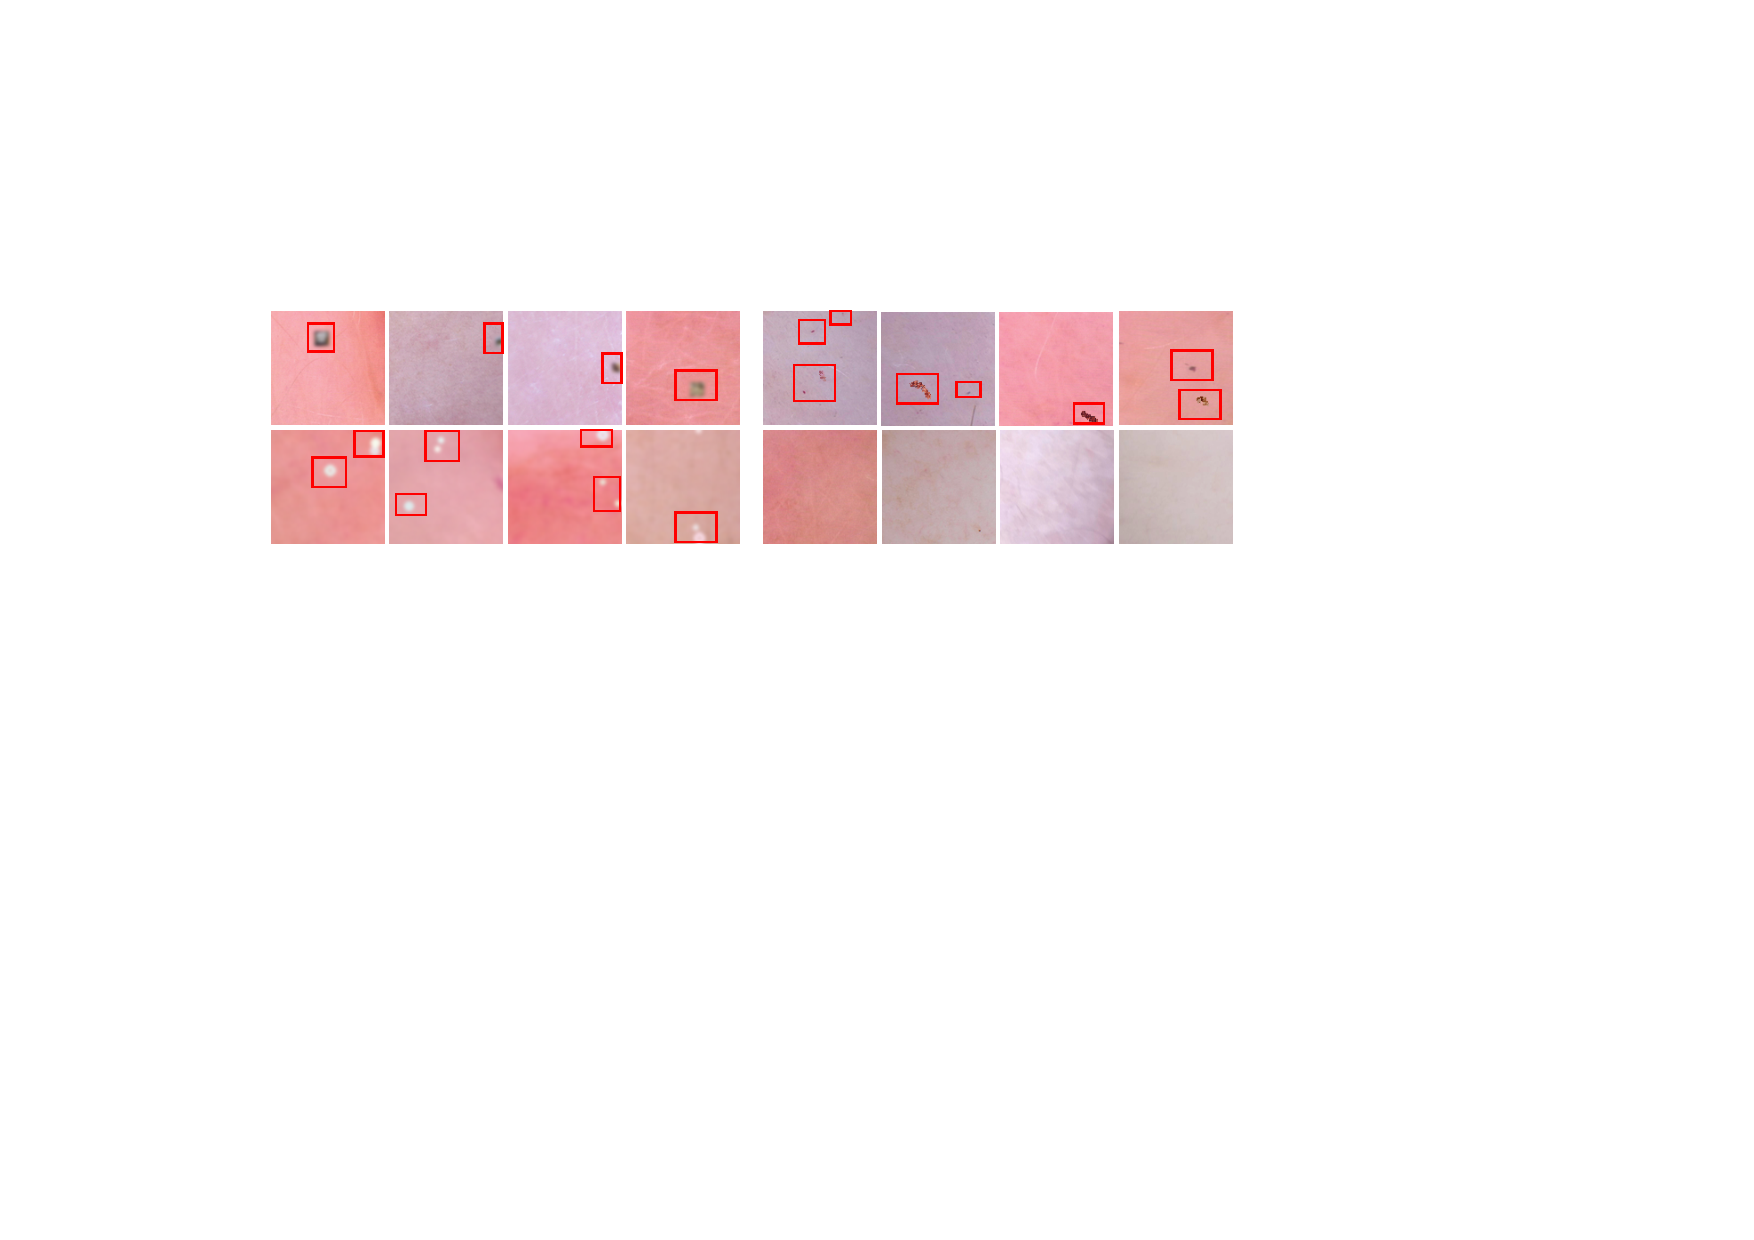
\includegraphics[width=1.0\textwidth]{figure/multi_classes_simulated_skin.pdf}
	\caption{多类模拟皮肤病病变数据集图像示例:按照从上到下,从左到右的顺序,第$1$行第$1$列到第$1$行第$4$列为皮肤图像加上经过局部模糊的Image-Net缩略图的异常图像(第一类异常);第$1$行第$5$列到第$1$行第$8$列为皮肤图像加上黑色素瘤区域的异常图像(第二类异常);第$2$行第$1$列到第$2$行第$4$列为皮肤图像加上经过局部模糊的圆环区域的异常图像(第三类异常);第$2$行第$5$列到第$2$行第$8$列为正常图像。异常图像中的生物标记物均已用红色矩形框标出。}
	\label{fig:mul_classes_simulated_ds}
\end{figure}

\section{实验设置}\label{sec:multi_classes_experiment_setting}
与上一章中二类问题所采用的相关实验设置相比,除超参数取值($\lambda_{1}=0.8,\lambda_{2}=10$)不同外,其他设置均相同。评价标准也与上一章相同(参见\ref{sec:exper_evaluation_metrics}小节),采用P-R曲线(多类模拟皮肤病病变数据集中三个异常类的像素数量统计表如\ref{tab:multi_ds_pixel_freqs}所示)作为实验评价标准。

如\ref{sec:difficulties}小节中所描述的那样,由于对抗生成网络中只有两个语义输入端(真/假),与二类问题不同的是,多类问题有多个异常类。为了解决这个多类异常与对抗生成网络本身性质的矛盾,我们将所有异常类看做一类,而正常类本身就作为另一类,从而将正常类看做对抗生成网络语义上的真,将所有异常图像看做对抗生成网络语义上的假。同时,取样时保持所有异常类之间的样本数量相等。在CNN分类器方面,我们直接将原来的二分类扩展到多分类,增加CNN分类器最后一个全连接层的输出维度,同时在训练CNN分类器时用多类交叉熵取代原来的二类交叉熵损失函数。本文提出模型的其他结构均与上一章相同。

\begin{table}[h]
	\centering
	\caption{多类模拟皮肤病病变数据集中的三类异常图像像素数量统计表。}
	\label{tab:multi_ds_pixel_freqs}
	\begin{tabular}{c|c|c|c}
		\toprule[2pt]
		数据集名称 & 正常像素数量 & 异常像素数量 & 比例 \\
		\midrule[2pt]
		第一类异常&  $21,222,487$ & $240,553$ & $\simeq 88: 1$ \\ \hline
		第二类异常&  $17,129,210$ & $90,374$ & $\simeq 190: 1$ \\ \hline
		第三类异常 & $17,341,855$ & $57,953$ & $\simeq 299: 1$ \\
		\bottomrule[2pt]
	\end{tabular}
\end{table}

\section{在多类模拟皮肤病病变数据集上的实验评估}\label{sec:multi_classes_experiments_res}
本文将展示本文提出模型在多类模拟皮肤病病变数据集上的实验结果,本文提出的模型同样将与CAM和Grad-CAM共计两种用于卷积神经网络可视化方法作定性分析和定量分析。下面展开相关内容的具体阐述。

\begin{figure}[H]
	\centering
	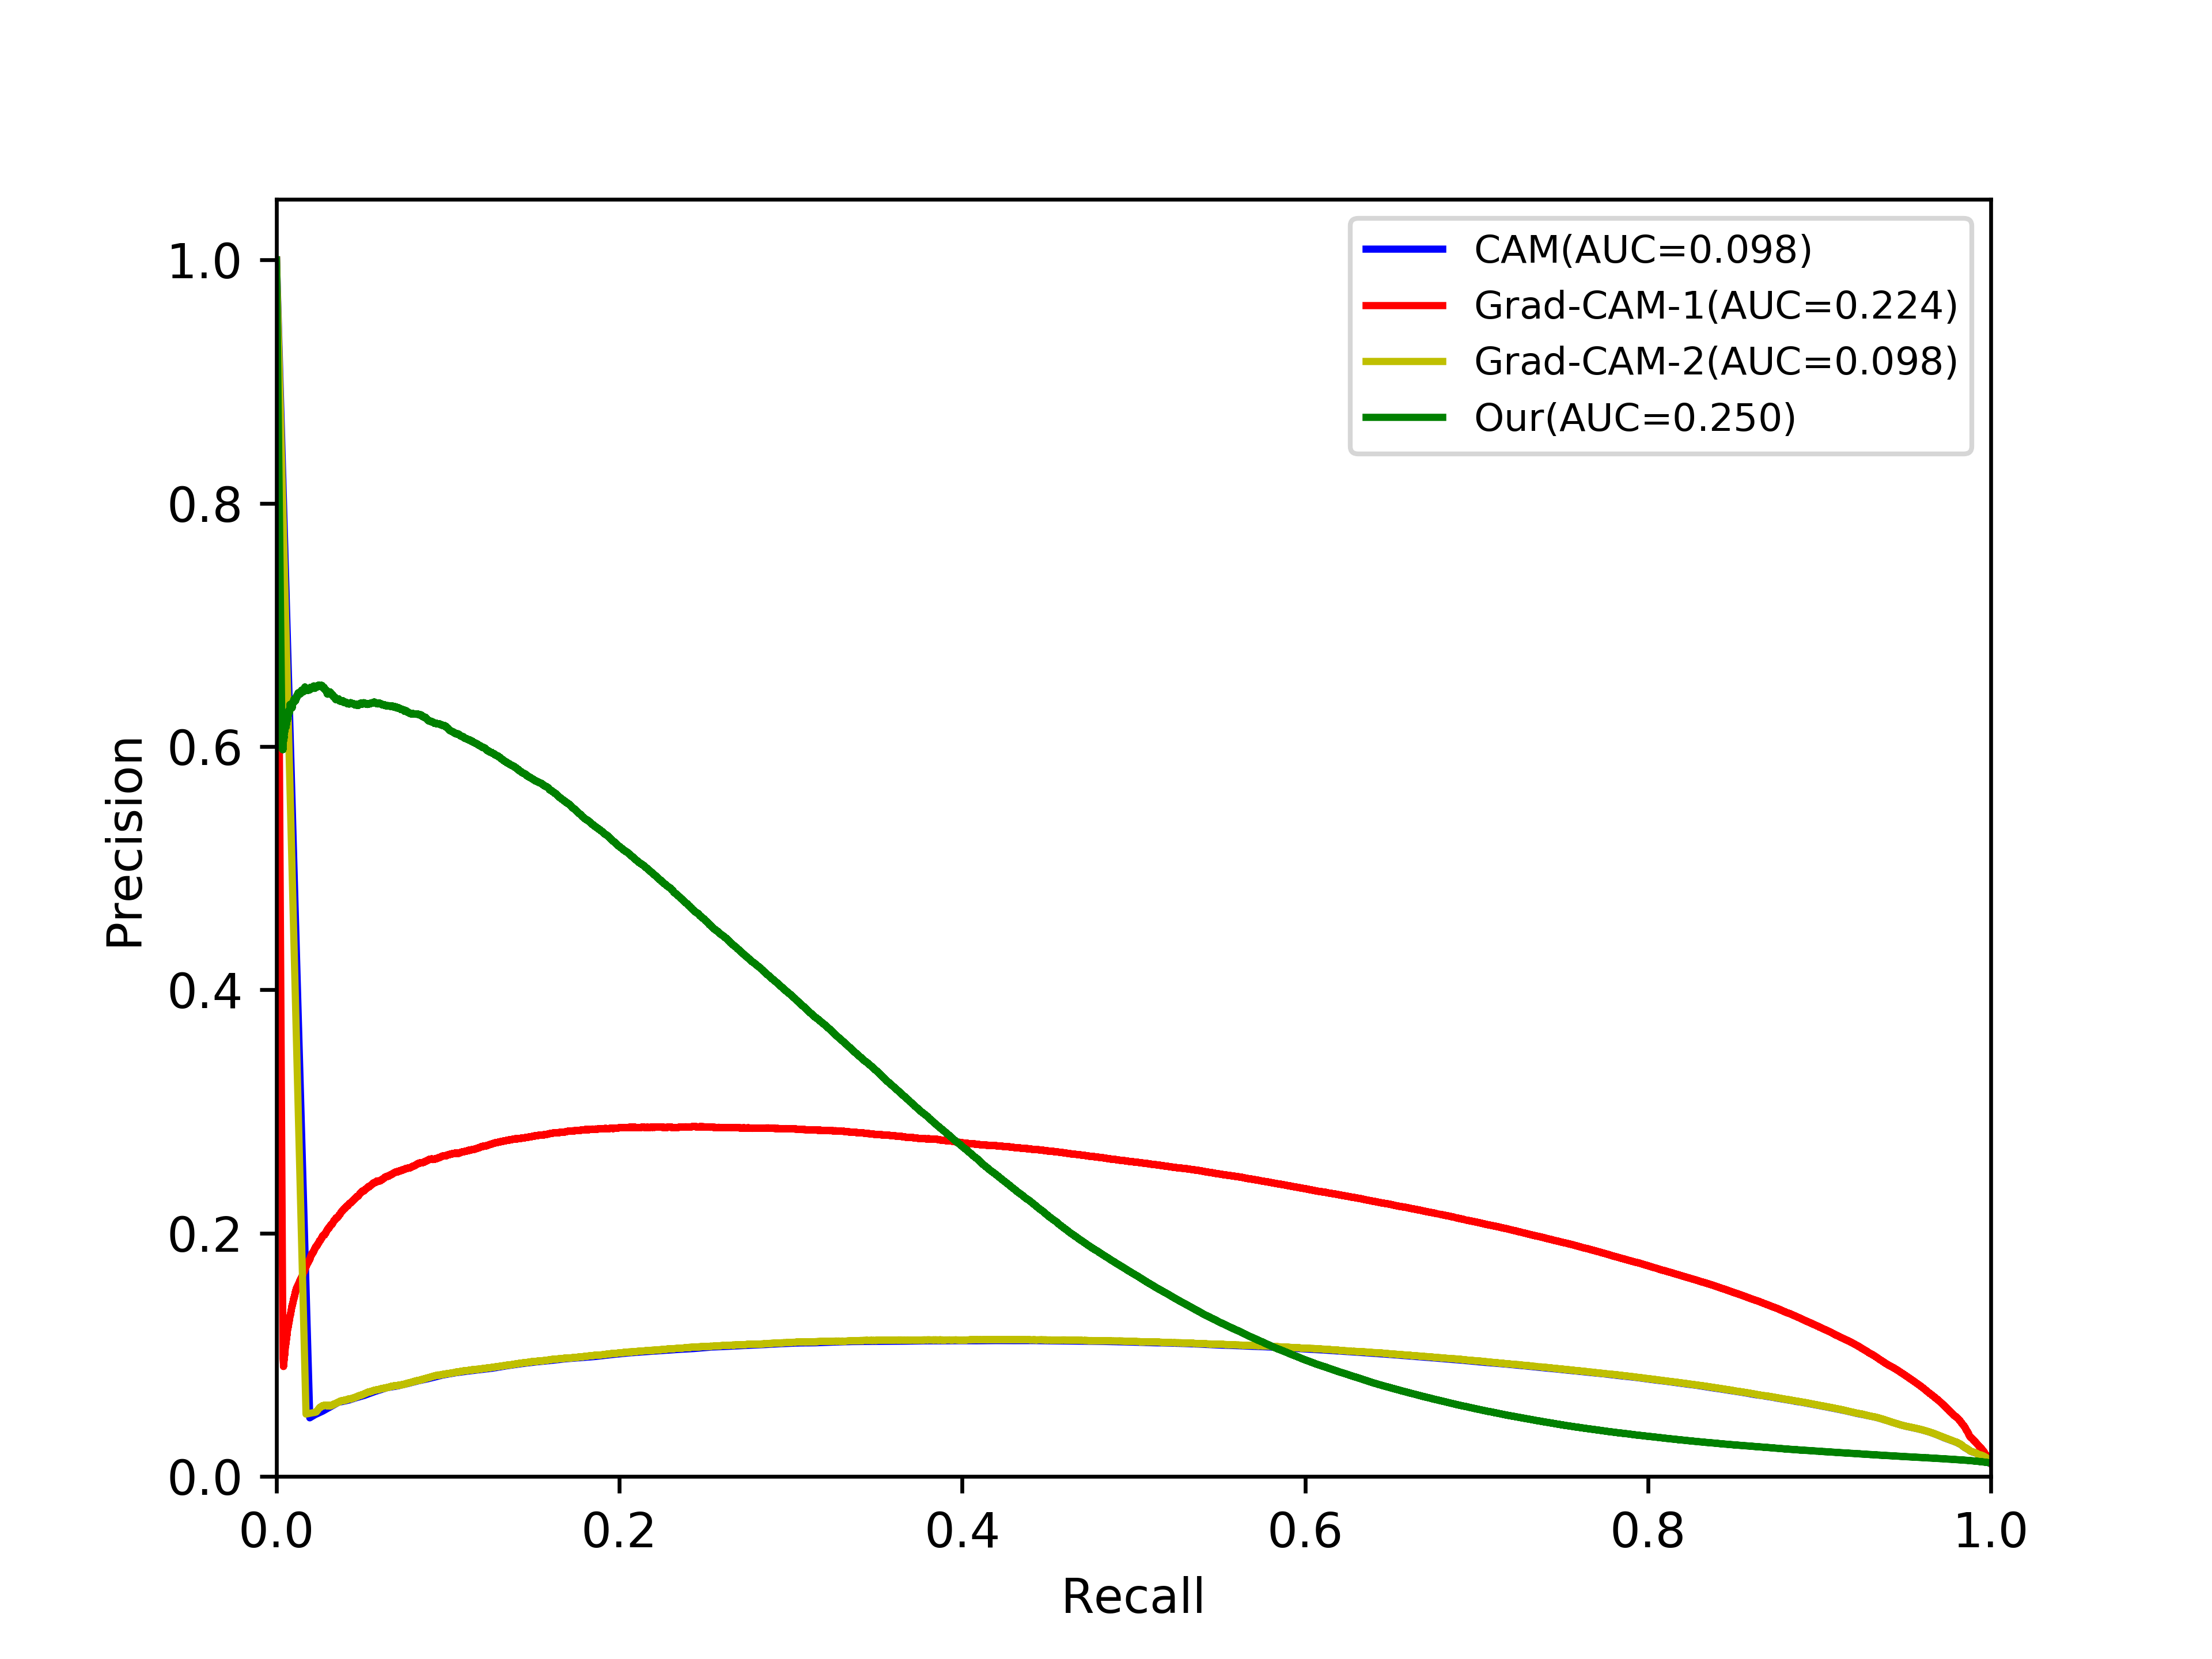
\includegraphics[width=1.0\textwidth]{figure/pr_curve_multi_skin/IMAGE_NET_pr_curve.png}
	\caption{CAM、Grad-CAM-1、本文提出的模型和Grad-CAM-2在多类模拟皮肤病病变数据集的第一类异常上画出的P-R曲线及其各自曲线下的面积(AUC,见右上角图例)。} 
	\label{fig:multi_simulate_pr_curve_image_net}
\end{figure}

\begin{figure}[H]
	\centering
	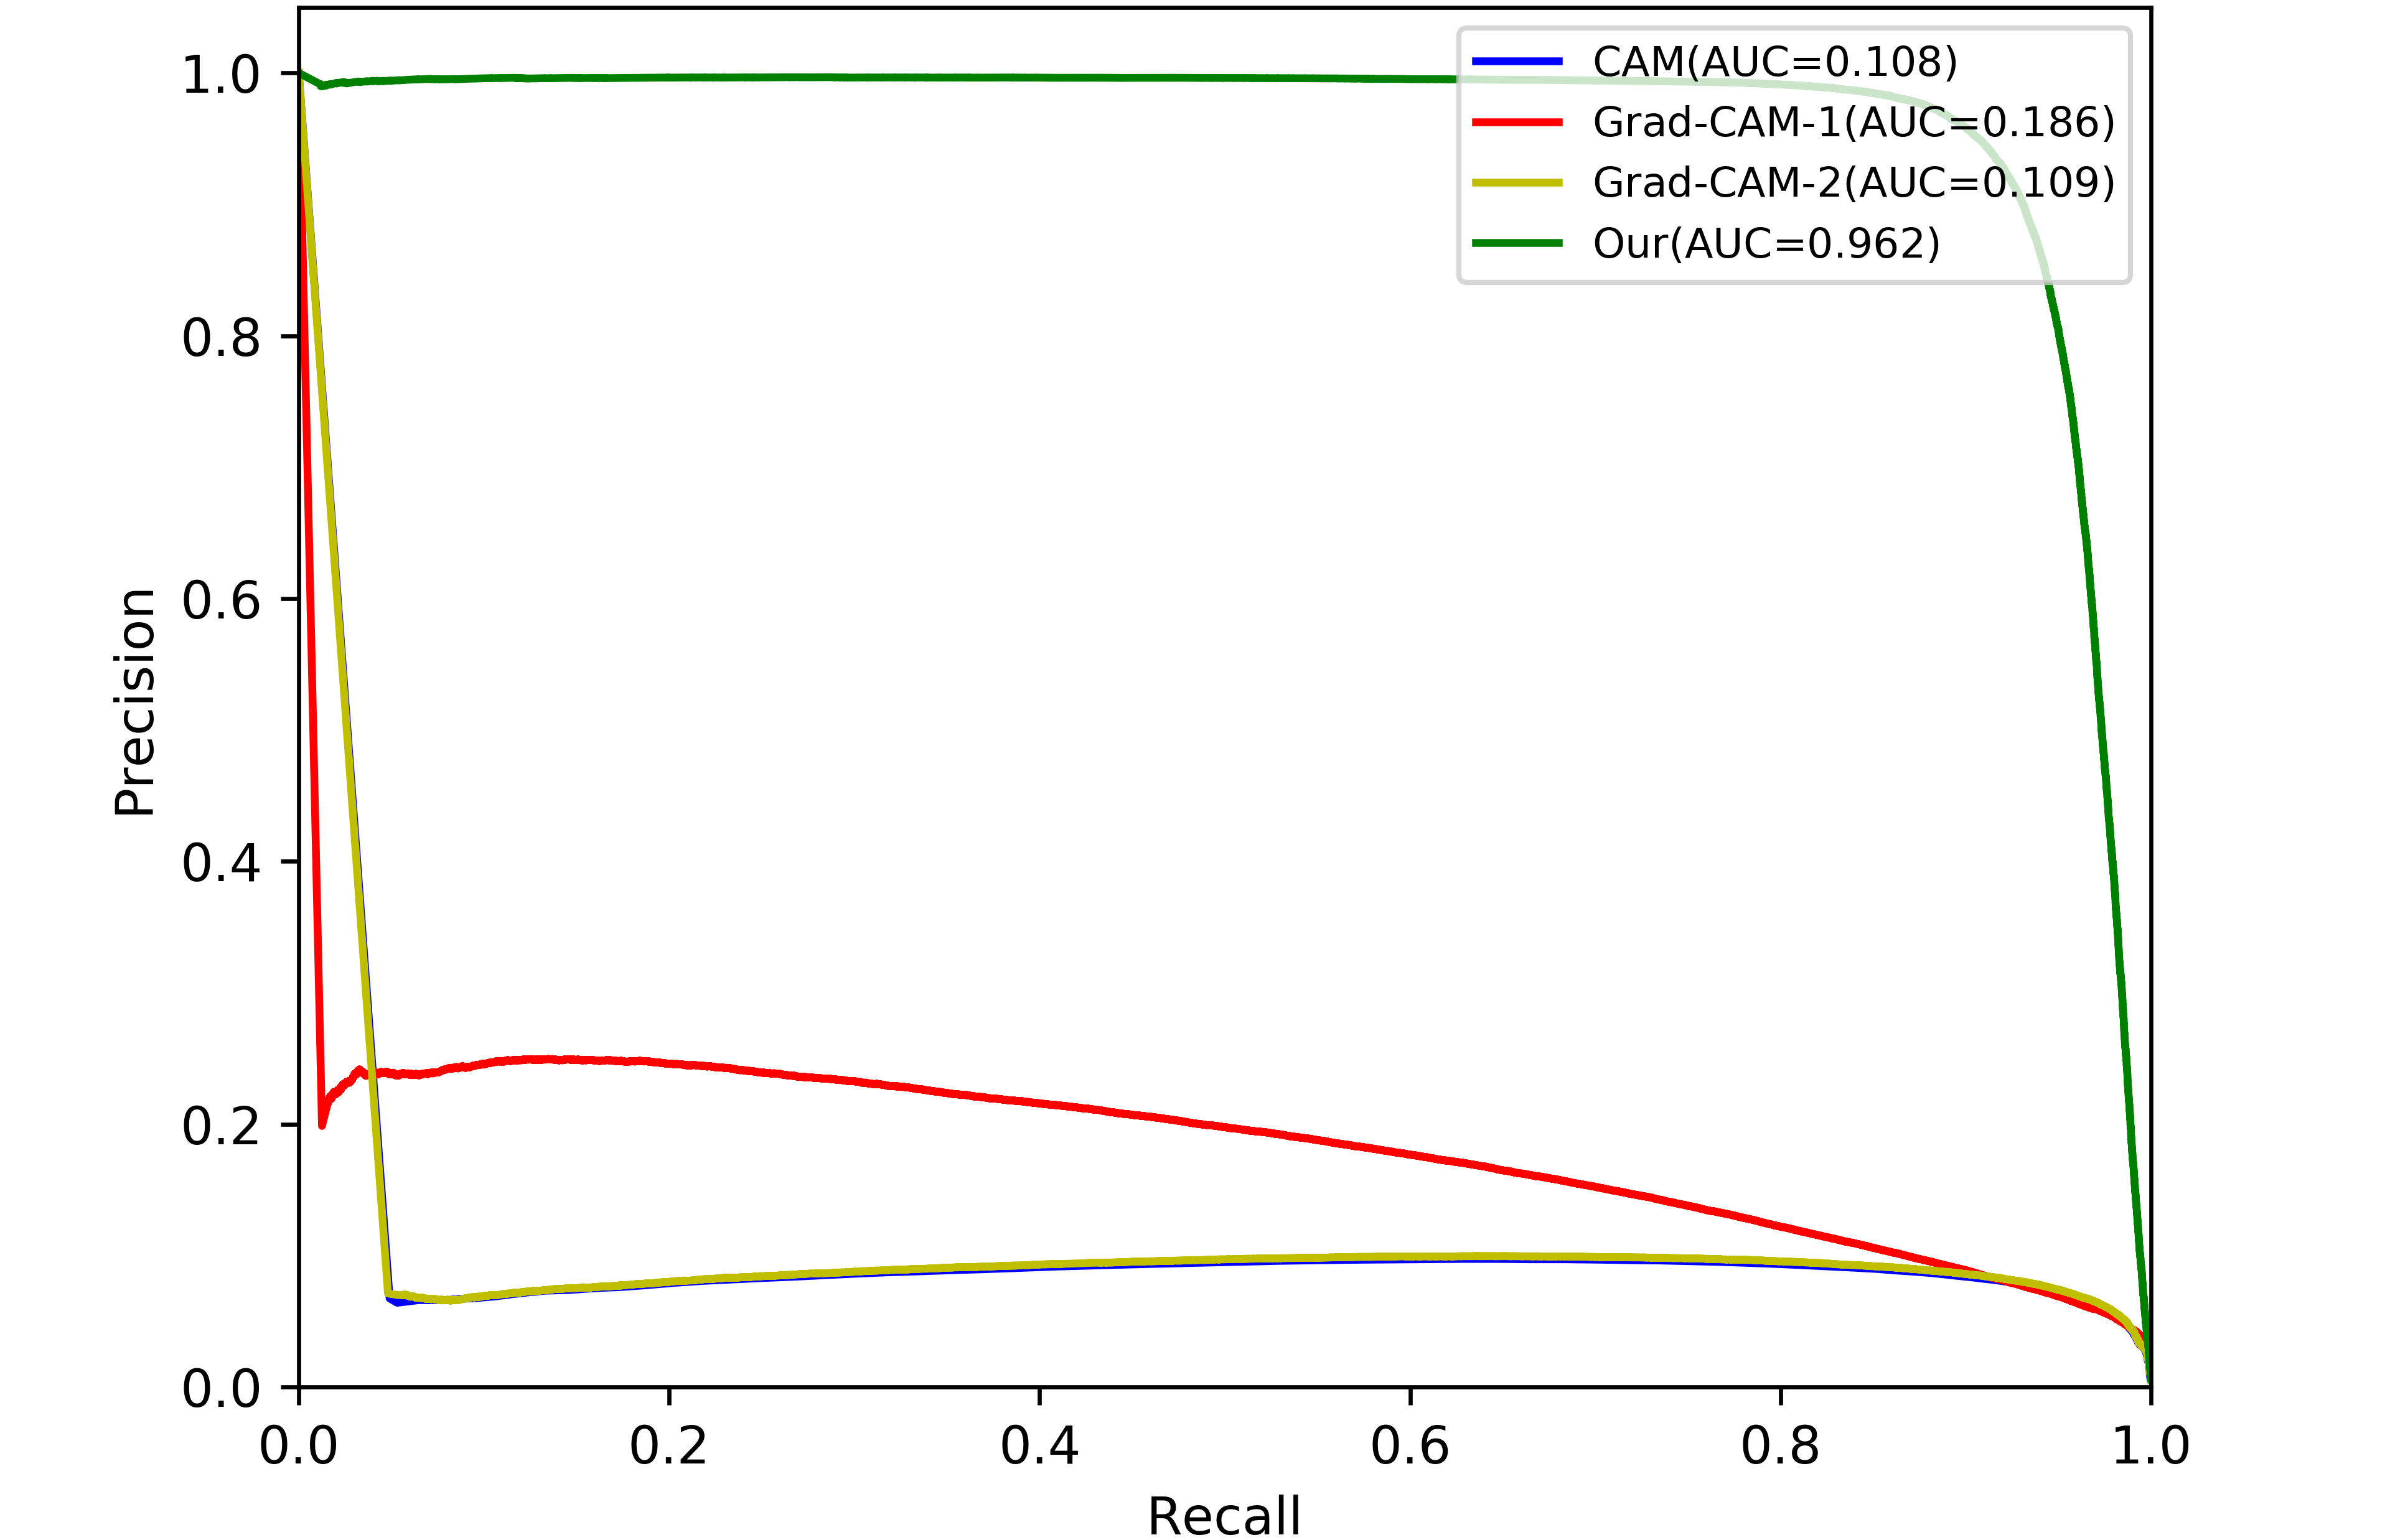
\includegraphics[width=0.95\textwidth]{figure/pr_curve_multi_skin/SKIN_pr_curve.png}
	\caption{CAM、Grad-CAM-1、本文提出的模型和Grad-CAM-2在多类模拟皮肤病病变数据集的第二类异常上画出的P-R曲线及其各自曲线下的面积(AUC,见右上角图例)。} 
	\label{fig:multi_simulate_pr_curve_skin}
\end{figure}
\vspace{-1.8cm}
\begin{figure}[H]
	\centering
	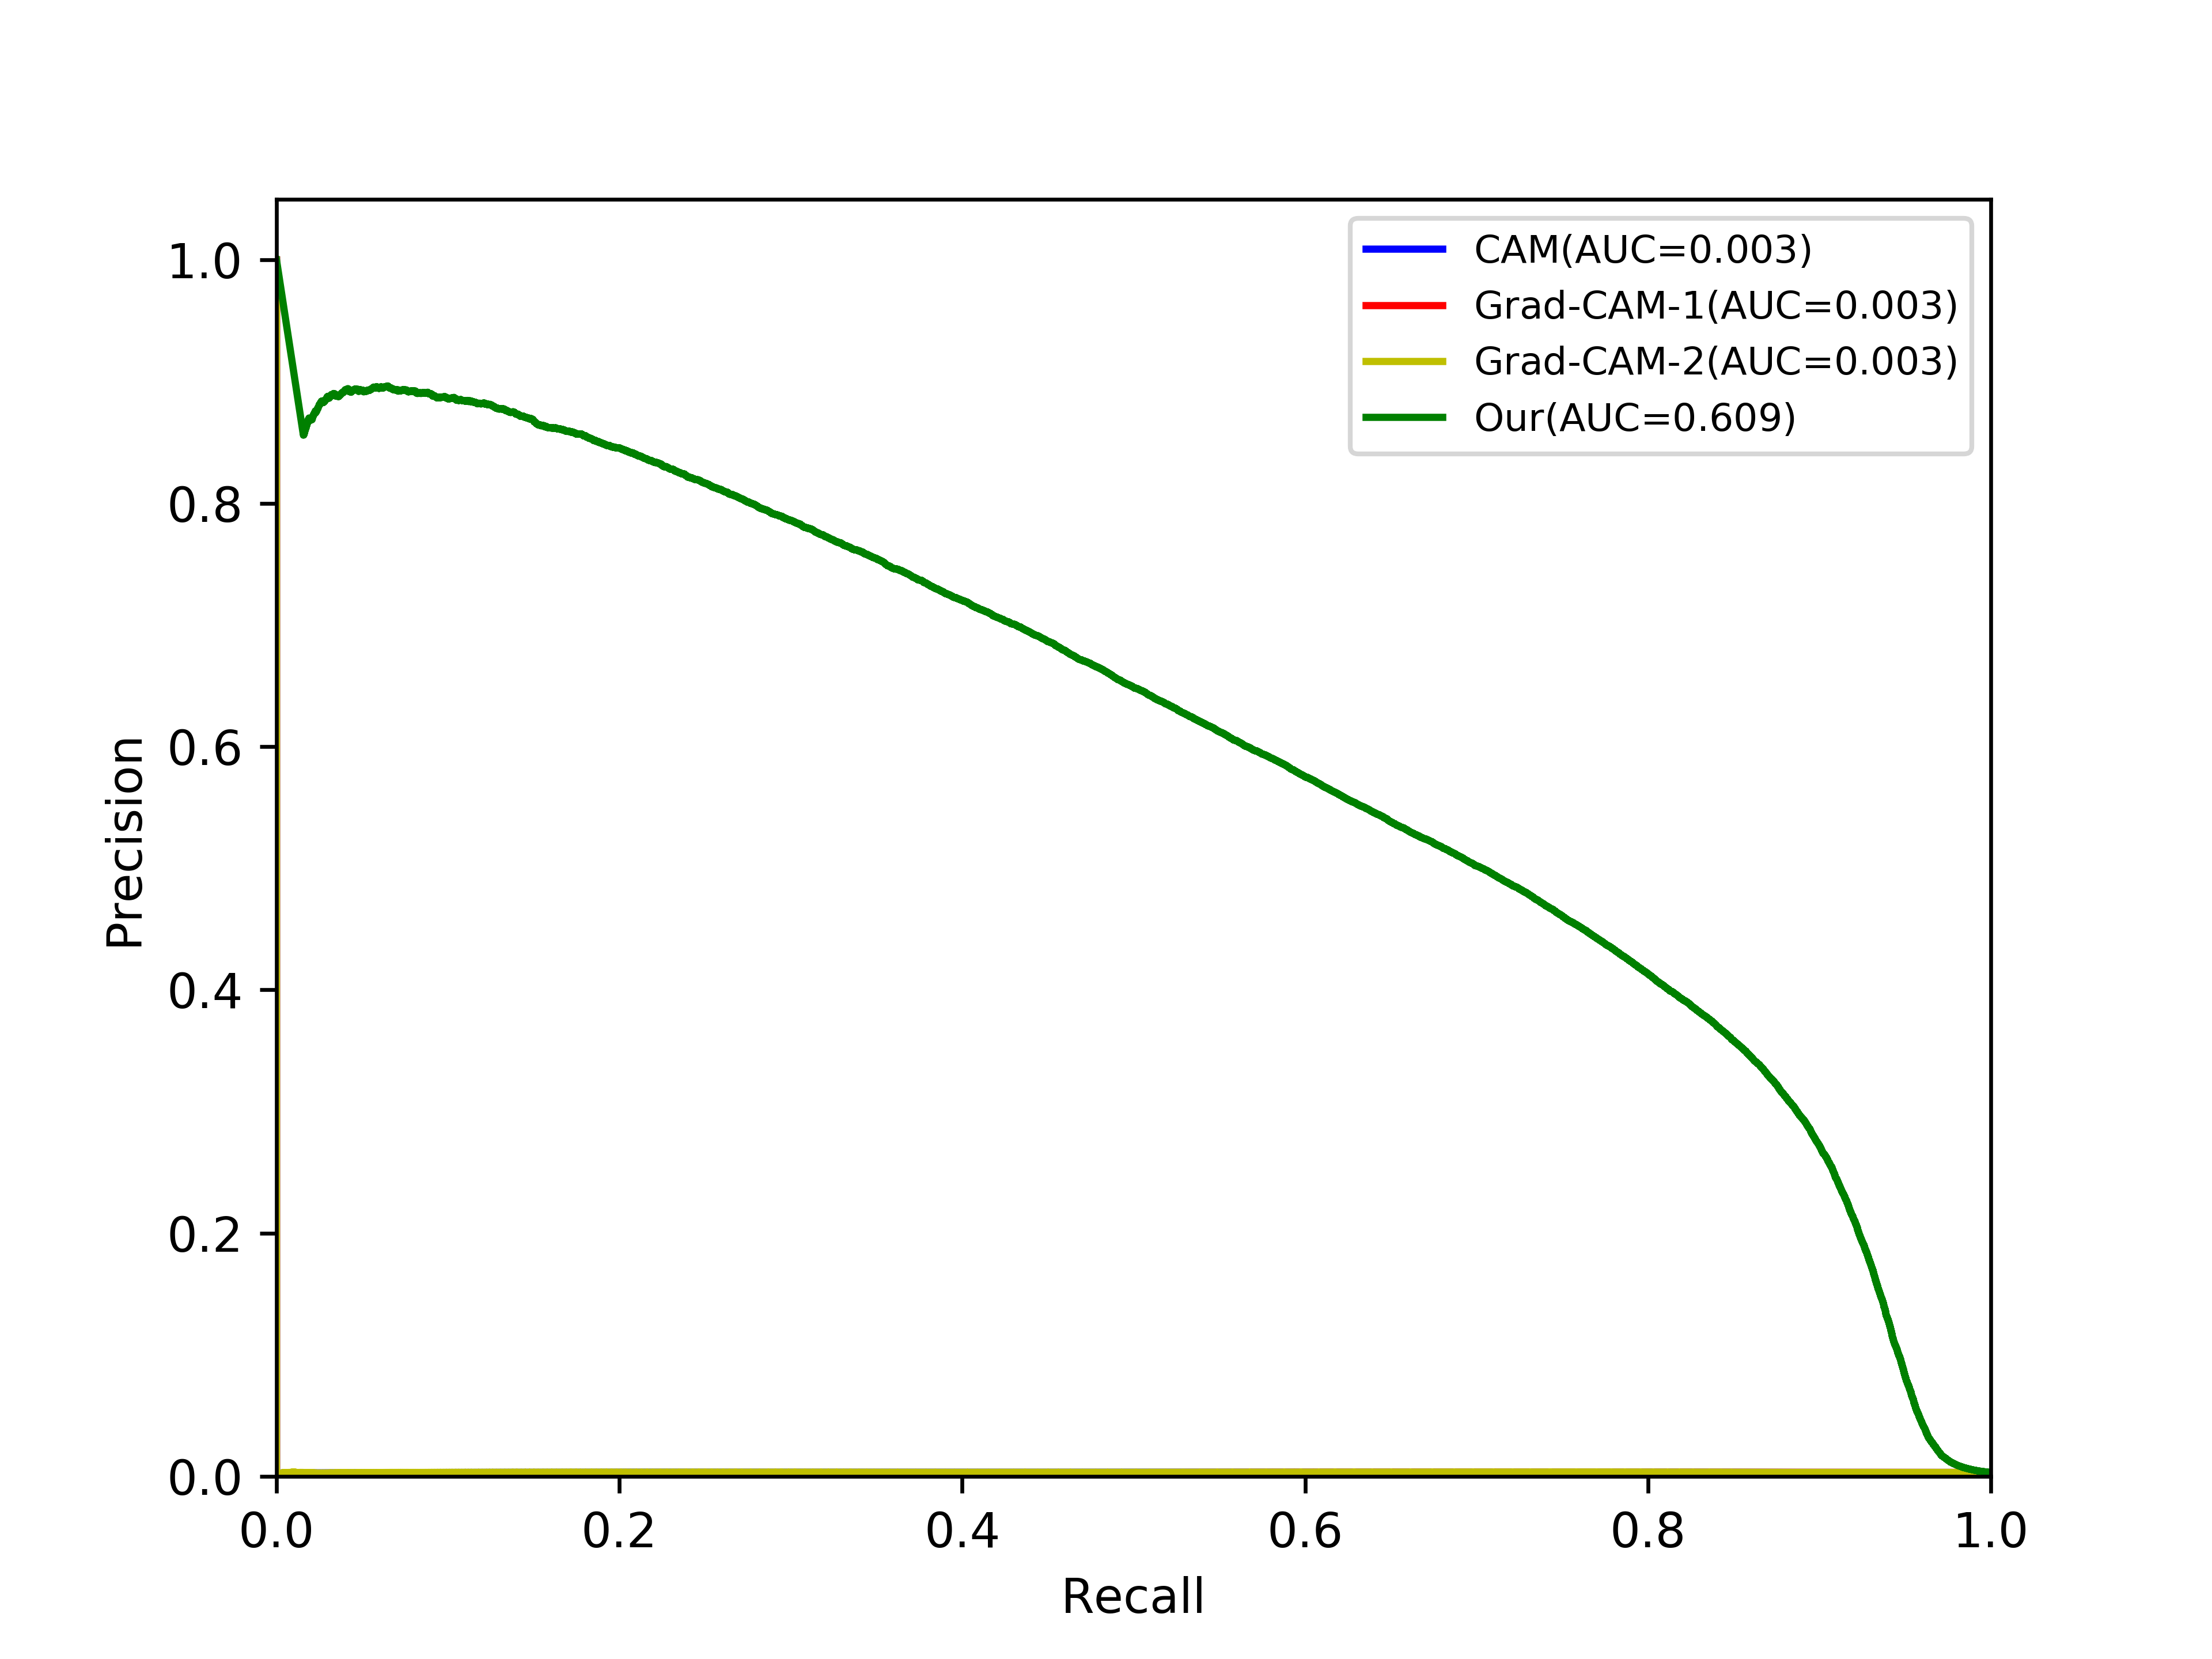
\includegraphics[width=0.95\textwidth]{figure/pr_curve_multi_skin/CIRCLE_pr_curve.png}
	\caption{CAM、Grad-CAM-1、本文提出的模型和Grad-CAM-2在多类模拟皮肤病病变数据集的第三类异常上画出的P-R曲线及其各自曲线下的面积(AUC,见右上角图例)。} 
	\label{fig:multi_simulate_pr_curve_circle}
\end{figure}


我们同样先训练得到了一个ResNet-18分类器,分类器最终的分类准确率达到了$99.9\%$,从而保证ResNet-18本身良好的分类性能。随后,与\ref{sec:bin_dr_ds_experiment}小节一样,我们分别使用CAM(见图\ref{fig:multi_simulated_skin_res}第$3$行)、Grad-CAM(见图\ref{fig:multi_simulated_skin_res}第$4$行和第$5$行)在多类模拟皮肤病病变数据集上完成了生物标记物的定位任务。
\begin{figure}[h]
	\centering
	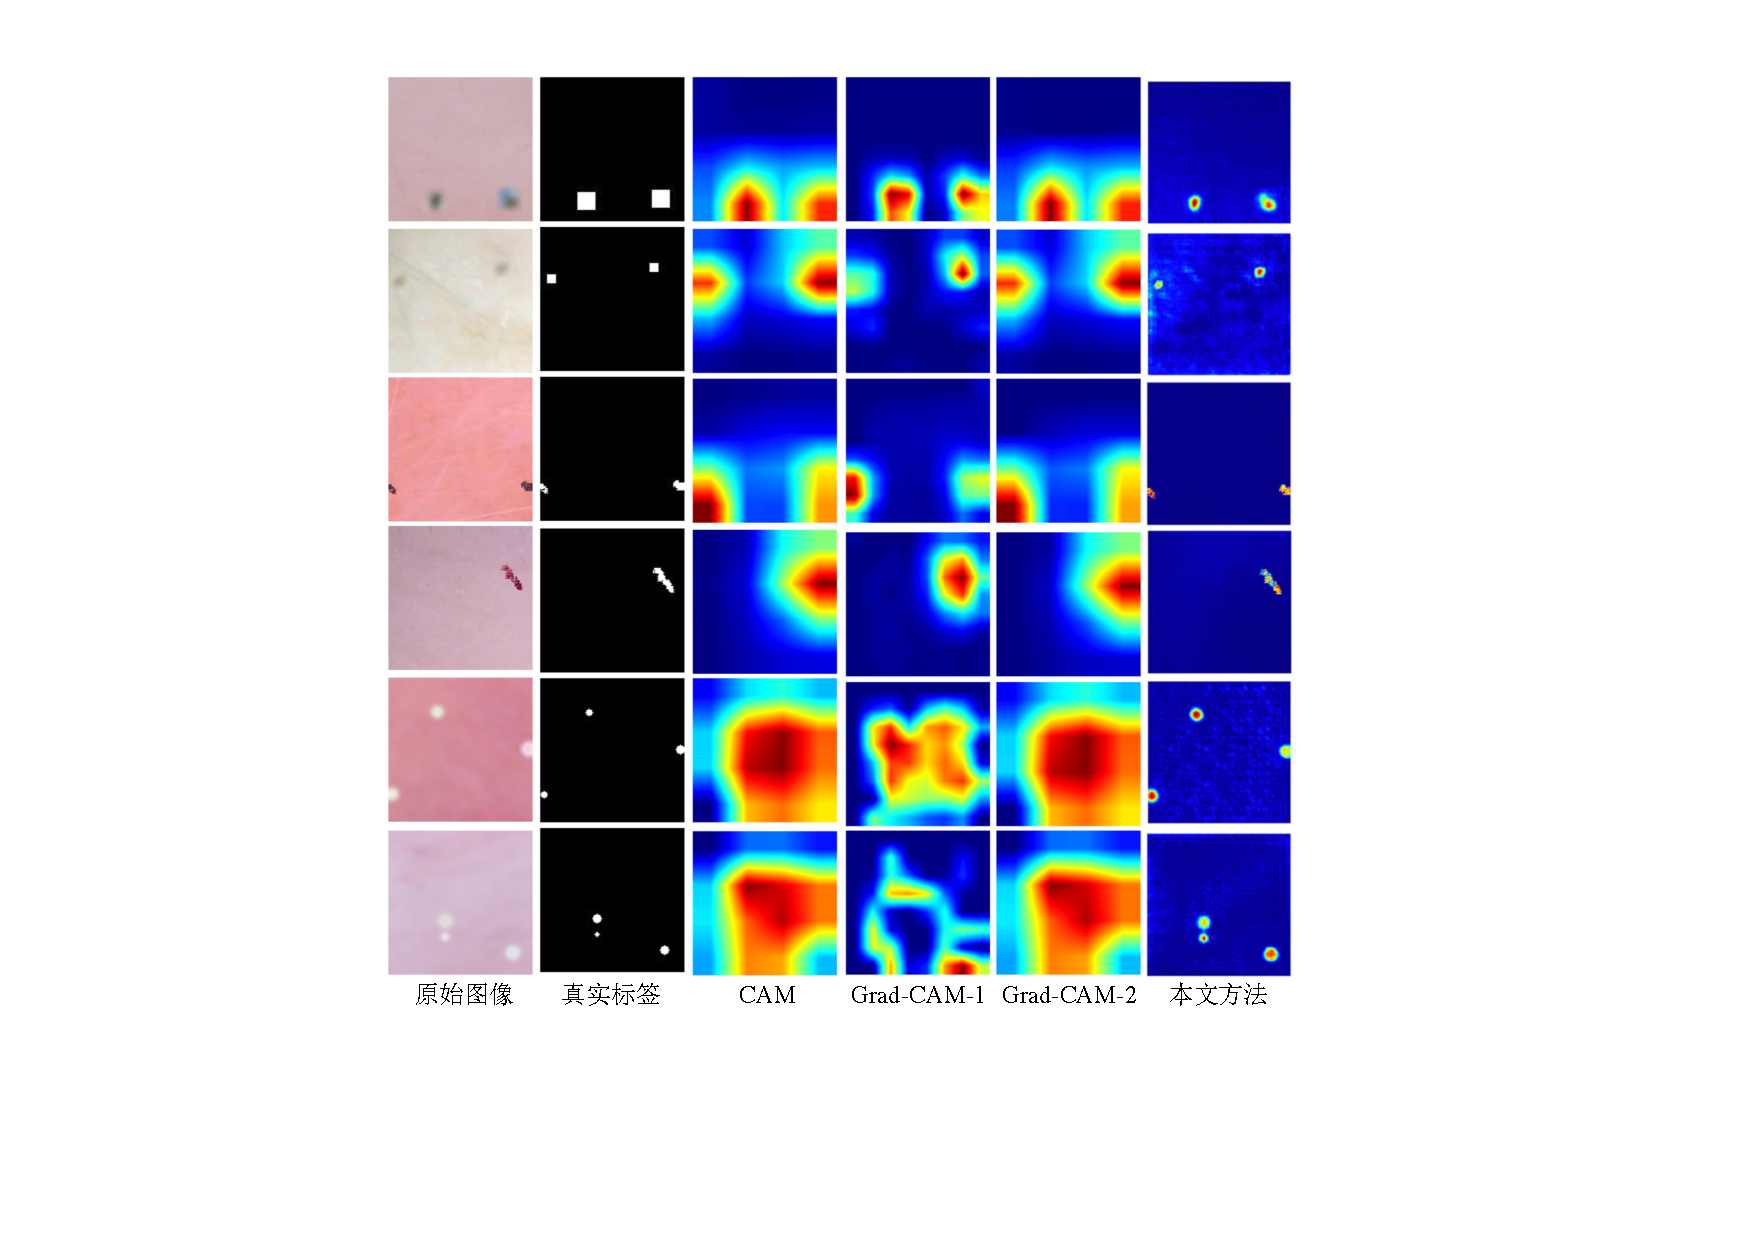
\includegraphics[width=1.0\textwidth]{figure/multi_simulated_skin_res.pdf}
	\caption{本文提出的模型在多类模拟皮肤病病变数据集上的定性评估:第$1-2$行、第$3-4$行和第$5-6$行分别为第一类异常、第二类异常和第三类异常图像实验结果。第$1$列表示该数据集中的原始图像,第$2$列表示原始的像素级标签。第$3$列表示CAM的定位结果,第$4$列表示Grad-CAM使用分类器中间层的特征图可视化结果(Grad-CAM-1),第$5$列表示Grad-CAM使用分类器最后一层特诊图可视化的定位结果(Grad-CAM-2),第$6$列表示本文提出模型的定位结果。}
	\label{fig:multi_simulated_skin_res}
\end{figure}

如图\ref{fig:multi_simulated_skin_res}所示,第$3$的定位结果标出的异常区域最多,虽然也包括了潜在的生物标记物,但是同时也将周边大量正常区域也误认作生物标记物。Grad-CAM作为CAM的扩展,对可视化层的选择更为灵活。如图中第$4$列和第$5$列分别选取中间卷积层和最后一层卷积层。可以发现,Grad-CAM-1取得了较为精确的结果,证明了其优于CAM的性能。另外,可以发现Grad-CAM-2给出的定位结果(第$5$列)与CAM(第$3$行)相差不大。与以上结果相比较,对于分散、形状各异的生物标记物,相比于CAM和Grad-CAM,本文提出的模型给出了更为精确的定位结果(第$6$行),从而从定性分析角度证明了本文提出的方法的性能优越性。


另外,由于多类模拟皮肤病病变数据集中的所有图像均存在像素级标注,本文还从定量角度对实验结果进行相关分析。由此,对于本文提出的模型、CAM、Grad-CAM-1和Grad-CAM-2,根据该数据集中的三类异常图像所绘制P-R曲线分别如图\ref{fig:multi_simulate_pr_curve_image_net}、图\ref{fig:multi_simulate_pr_curve_skin}和图\ref{fig:multi_simulate_pr_curve_circle}所示。不难发现,绿色P-R曲线(本文提出的方法)在其他三条曲线的上方,且与下侧横轴和左侧纵轴围成的封闭区域面积显然最大。在第一类异常、第二类异常和第三类异常上,本文提出的方法均取得了最高的AUC分数,在三类异常上计算得到的AUC分数分别为$0.250$(见图\ref{fig:multi_simulate_pr_curve_image_net})、$0.870$(见图\ref{fig:multi_simulate_pr_curve_skin})和$0.609$(见图\ref{fig:multi_simulate_pr_curve_circle}),从而从定量角度说明本文提出的方法相较于CAM和Grad-CAM具有更为出色的性能表现。以上四种方法更为直观的AUC分数如表\ref{tab:multi_ds_auc_scores}所示。


\begin{table}[!htbp]
	\centering
	\caption{本文提出的方法、CAM、Grad-CAM-1和Grad-CAM-2在三类异常图像上计算得到的AUC分数及其平均。}
	\label{tab:multi_ds_auc_scores}
	\begin{tabular}{c|c|c|c|c}
		\toprule[2pt]
		& CAM & Grad-CAM-1 & Grad-CAM-2 & 本文提出的方法 \\
		\midrule[2pt]
		第一类异常&$0.098$ & $0.224$ &  $0.098$ & $\textbf{0.250}$ \\ \hline
		第二类异常&  $0.108$ &$0.186$ & $0.109$ & $\textbf{0.870}$ \\ \hline
		第三类异常 & $0.003$ & $0.003$ & $0.003$ & $\textbf{0.609}$ \\ \hline
		Average AUC & $0.070$ & $0.138$ & $0.070$ & $\textbf{0.576}$ \\ 
		\bottomrule[2pt]
	\end{tabular}
\end{table}

\section{对于经过编码器-解码器的多类模拟皮肤病病变图像的定量分析}
在本节中,本文同样将设置一组实验从间接角度证明本文提出的模型能够较好去除异常图像中的生物标记物或者异常区域。与\ref{sec:indirect_quantitative_evaluation}小节中的设计思想相同,在理想情况下,如果一种方法能够完全定位并去除生物标记物,则去除生物标记物之后的图像不再包含生物标记物,则这些图像将很难与正常图像分开。根据以上前提假设,我们将多类模拟皮肤病病变数据集按照$80\%$和$20\%$的比例将其分为训练集和测试集(下文简称为“原始四类数据集”),随后用训练集训练一个ResNet-18四分类器。接着,我们将原始多类数据集中的每一张图像作为输入送入编码器-解码器,并将输出收集起来,这样我们得到一个新的数据集(下文简称为“‘正常’四类数据集”)。最后,我们用上述ResNet-18对“正常”多类数据集中的每一张图像进行分类。在评价标准方法,与\ref{sec:indirect_quantitative_evaluation}小节不同的是,我们不选定Recall和Specificity作为评价标准,这是因为多类问题中异常图像作为输入经过编码器-解码器之后的输出可能会向其他异常类转变而二类问题中异常图像作为输入经过编码器-解码器之后的输出只能向正常图像转变。因此,对于正常图像,我们希望编码器-解码器的输出中尽量少的图像被ResNet-18判别为异常;而对于异常图像,我们希望编码器-解码器的输出中尽量多的图像被ResNet-18判别为异常。因此,编码器-解码器对于正常图像输入的保持能力可定义为:

\begin{equation}\label{equ:normal_imgs_kep_rate}
\text{正常类的转化率}=\frac{\text{输出图像中被判定为异常的图像数量}}{\text{输入正常图像的数量}}.
\end{equation}

\noindent 同理,编码器-解码器对于异常图像输入的转化能力可定义为:

\begin{equation}\label{equ:lesion_imgs_converted_rate}
\text{异常类的转化率}=\frac{\text{输出图像中被判定为正常的图像数量}}{\text{输入异常图像的数量}}.
\end{equation}

\noindent 显然,正常类的转化率越低而异常类的转化率越高表示模型定位并去除生物标记物的能力越强。相关实验结果如表\ref{tab:quantitative_simulated_skin}所示。

\begin{table}[h!]
	\centering
	\caption{原始四类数据集和“正常”四类数据集在ResNet-18分类器上的分类结果。前两列表示在原始四类数据集上的实验结果,后两列表示“正常”四类数据集上的实验结果。} 
	\label{tab:quantitative_simulated_skin}
	\begin{tabular}{c|cc|cc}
		\toprule[2pt]
		& \multicolumn{2}{c|}{\shortstack{原始四类数据集\\\scriptsize{(分类正确率)}}} &\multicolumn{2}{c}{\shortstack{“正常”四类数据集\\\scriptsize{(保持率)}}} \\
		&  训练集 & 验证集 & 训练集 & 验证集\\
		\midrule[2pt]
		正常类 & $0.992$ & $0.989$ & $0.094$ & $0.097$\\ \hline
		第一类异常 & $0.985$ & $0.981$ & $0.753$ & $0.741$\\ \hline
		第二类异常 & $0.999$ & $0.986$ & $0.976$ & $0.981$\\ \hline
		第三类异常 & $1.000$ & $1.000$ & $0.856$ & $0.840$\\
		\bottomrule[2pt]
	\end{tabular}
\end{table}

我们可以从表\ref{tab:quantitative_simulated_skin}中前两列看出,对于原始四类数据集,无论是正常类还是三个异常类,训练集和测试集上分类正确率均达到了$98\%$,这表明ResNet-18四类分类器可以很好学习到生物标记物的相关特征。而在该表的后两列中,我们可以发现,对于三个异常类,异常图像的转化率都比较高(第一类异常,训练集和测试集上的转化率分别为$75.3\%$和$74.1\%$),尤其是第二类异常,训练集和测试集上的转化率分别达到了$97.6\%$和$98.1\%$,以上结果可表明编码器-解码器对于异常图像输入有较好的转化能力,可以很好的定位并去除生物标记物。相比之下,正常类的转化率要低得多,在训练集和测试集上的转化率分别为$9.40\%$和$9.70\%$,这可以说明编码器-解码器对于正常图像输入有较好的保持能力。

\begin{figure}[h]
	\centering
	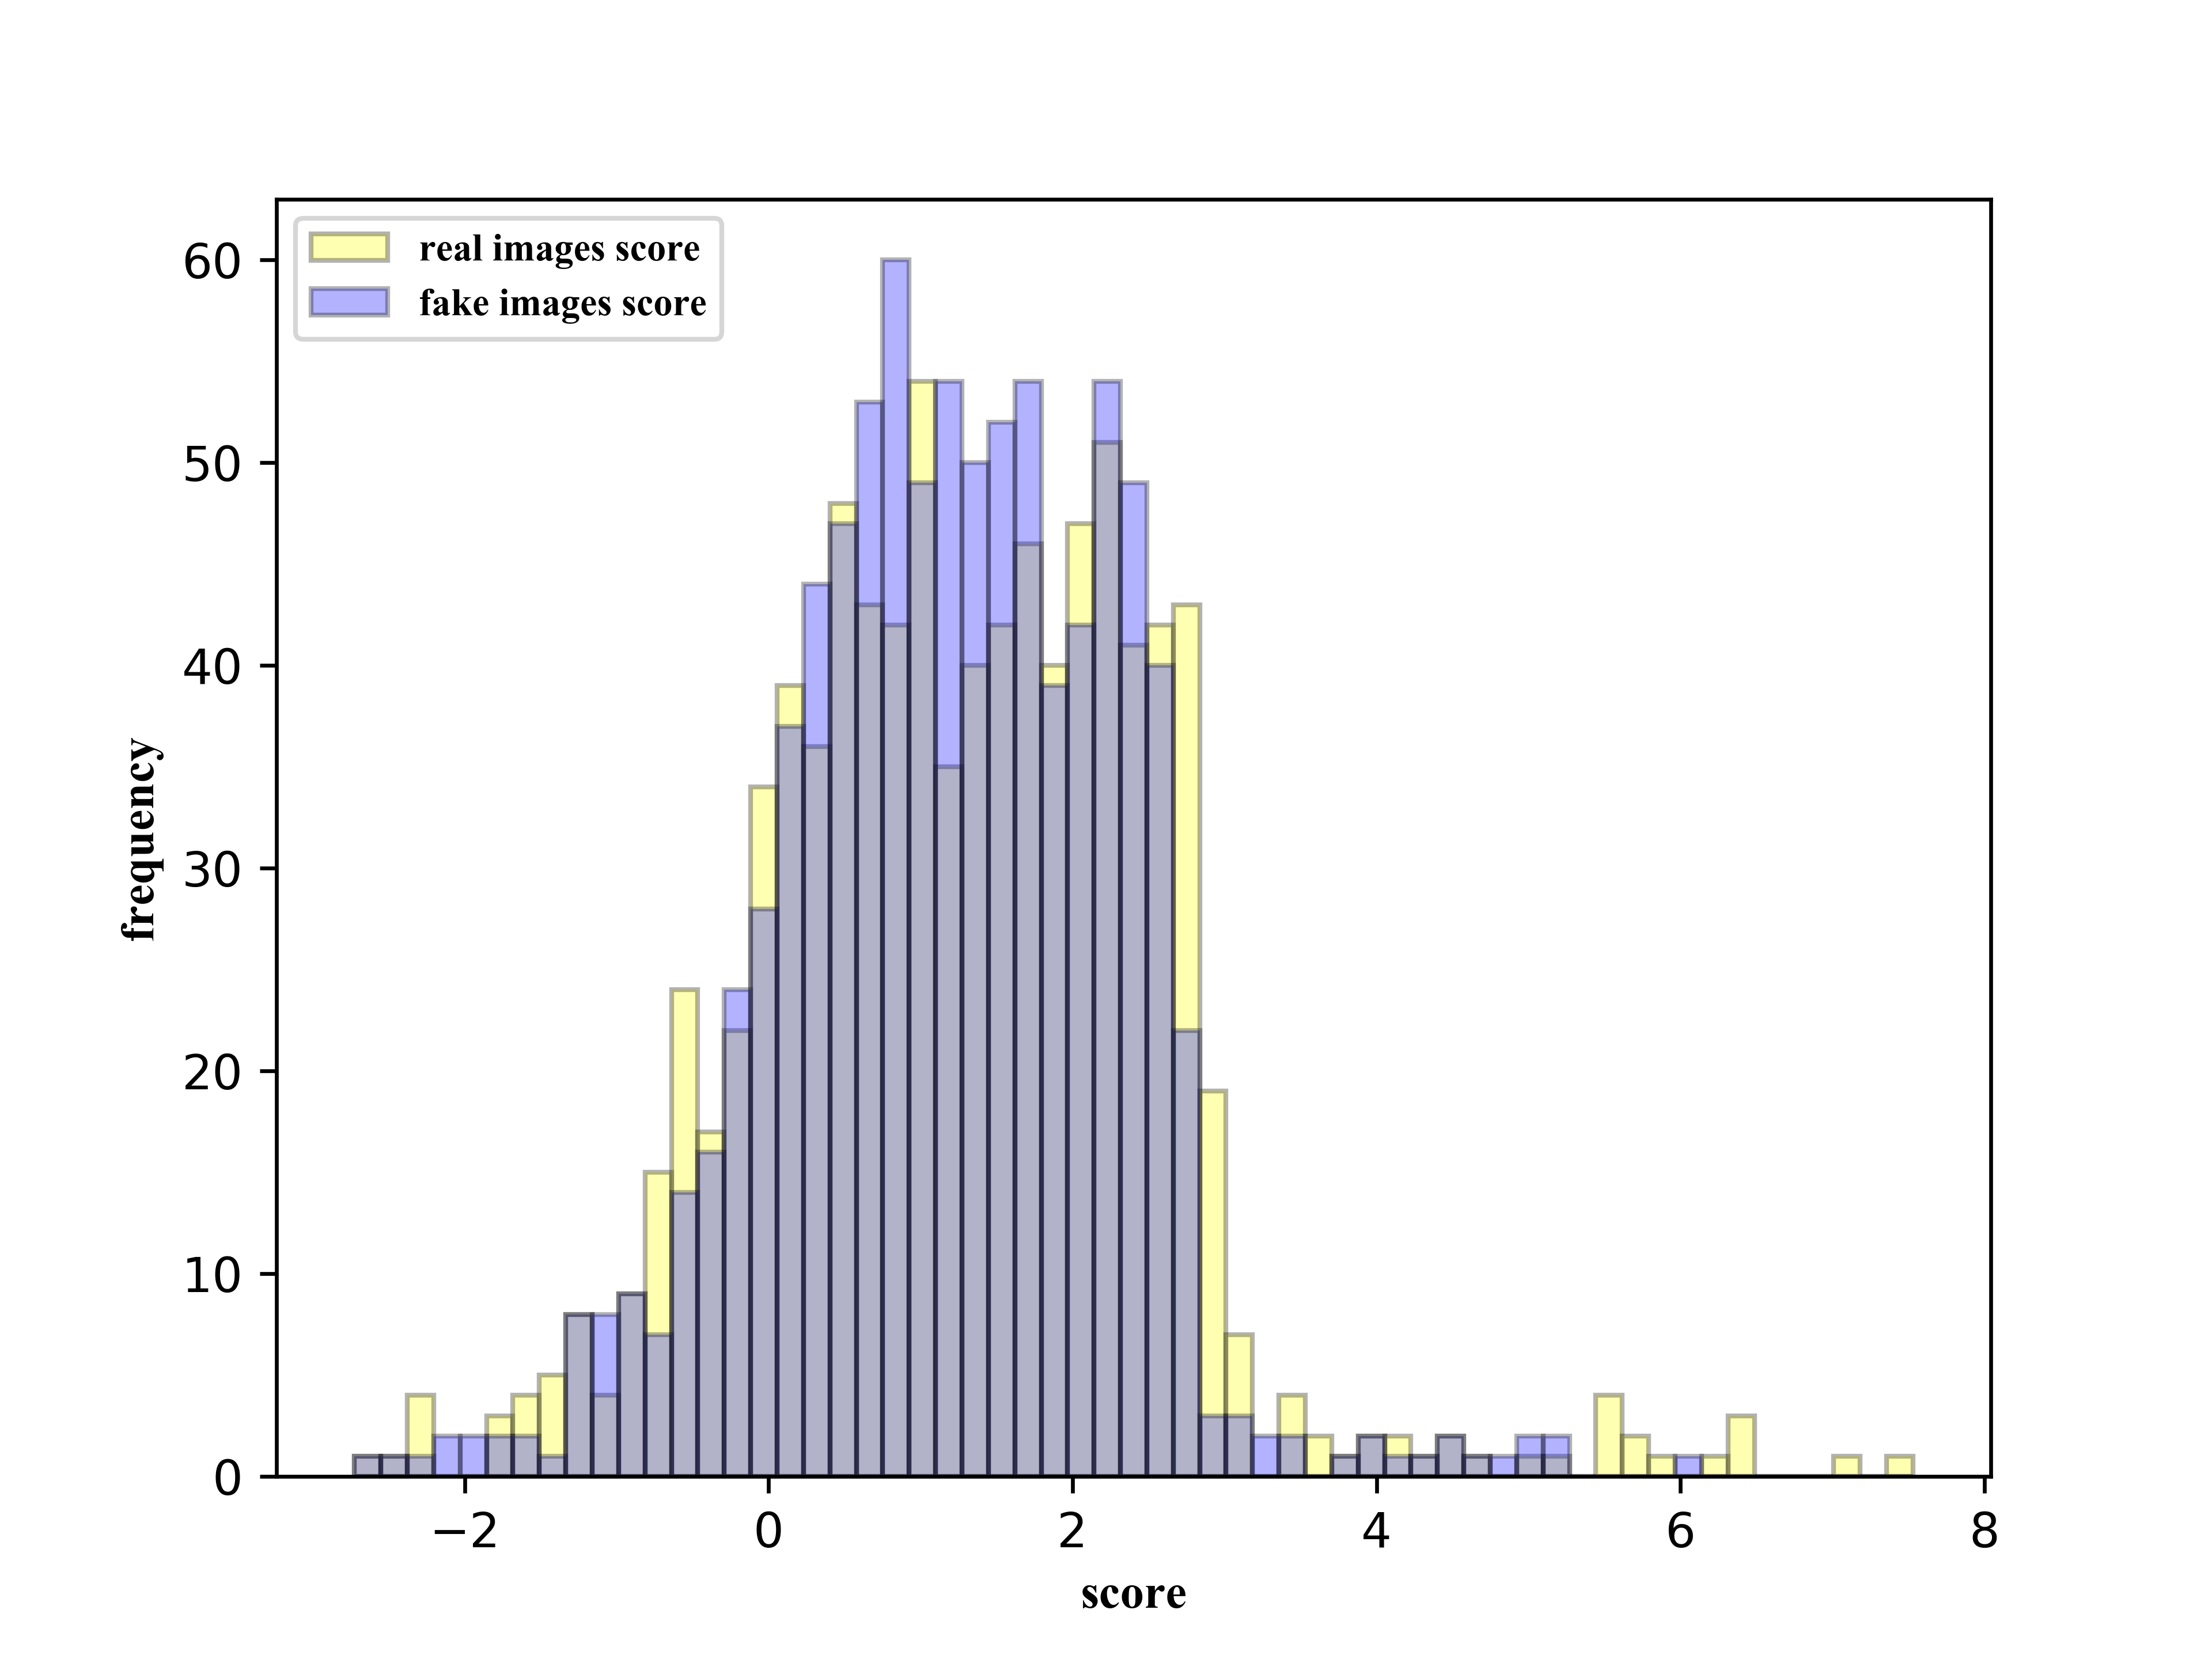
\includegraphics[width=1.0\textwidth]{figure/simulated_skin_score_distribution.png}
	\caption{将原始数据集中的正常图像和“正常”数据集中的“正常”图像分别送入到判别器之后,根据输出分数绘制的频率分布直方图。黄色柱子表示判别器真图像输入端的输出分数,紫色柱子表示判别器假图像输入端的输出分数,灰色柱子表示以上两者的重叠部分。}
	\label{fig:simulated_skin_hist_freq}
\end{figure}

以上实验从额外训练的ResNet分类器简介说明本文提出的模型在定位并去除生物标记物方面具有较强能力。在本小节中,我们还将“正常”四类数据集中的正常图像和异常图像均送入判别器,从而从判别器角度再次验证上述结论,判别器输出分数的频率分布直方图如图\ref{fig:simulated_skin_hist_freq}所示。从图\ref{fig:simulated_skin_hist_freq}中我们可以发现根据判别器两端输出分数所绘制的频率直方图中有较大重叠面积。另外,根据以上频率直方图,我们计算得到判别器两端输出分数的平均数分别为$1.3 $和$1.2$。而初试参数下,我们计算得到判别器两端输出的平均分数分别为$2.5$和$-0.5$,这说明在训练结束后,判别器输出两端输入图像的相似性得到了极大提升(平均分数差距:$3.0\rightarrow 0.1$),进一步说明判别器很难分辨输入图像的真/假,从而证明编码器-解码器的异常图像输出已经十分接近正常图像输出,由此我们可以推断出编码器-解码器已经很好的定位并去除了异常图像中的生物标记物。

\section{不同超参数下的实验结果分析}\label{sec:multi_classes_hyper_paras}
在本小节中,本文将探究。


\begin{figure}[!htbp]
	\centering
	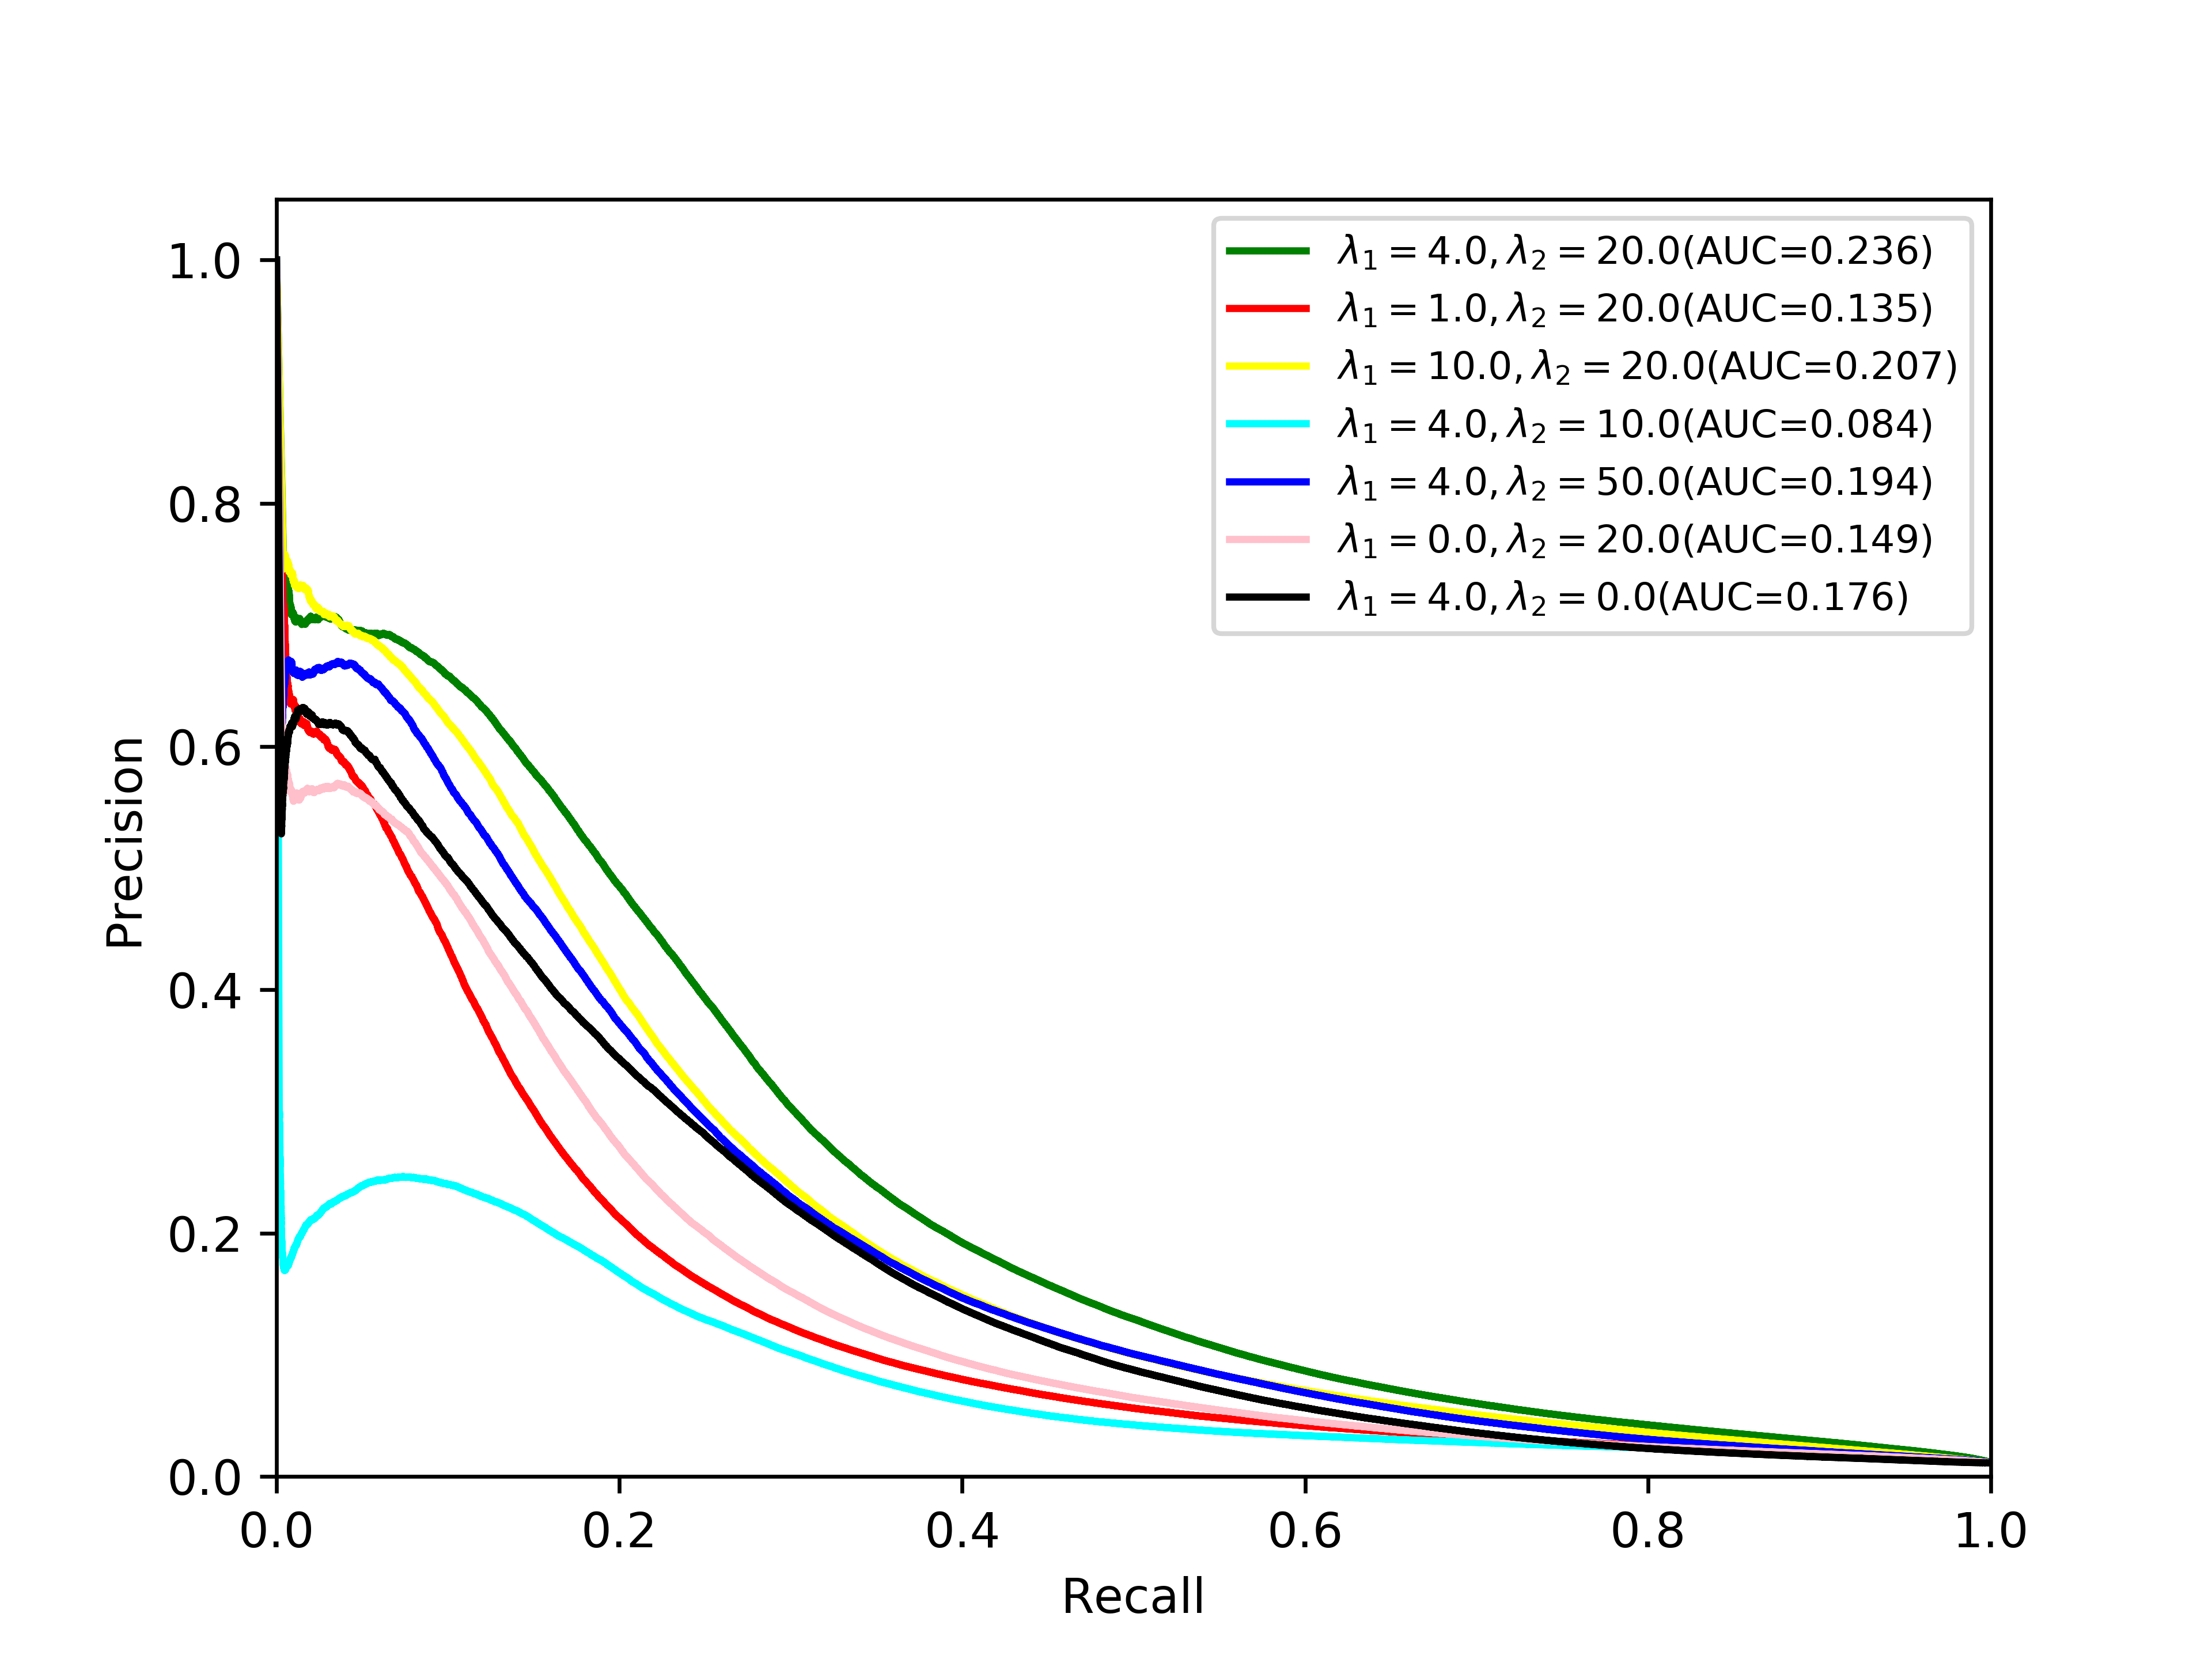
\includegraphics[width=1.0\textwidth]{figure/pr_curve_multi_skin_hyper_paras/IMAGE_NET_pr_curve.png}
	\caption{CAM、Grad-CAM-1、本文提出的模型和Grad-CAM-2在多类模拟皮肤病病变数据集的第一类异常上画出的P-R曲线及其各自曲线下的面积(AUC,见右上角图例)。} 
	\label{fig:multi_simulate_pr_curve_image_net_hyper_paras}
\end{figure}

\begin{figure}[!htbp]
	\centering
	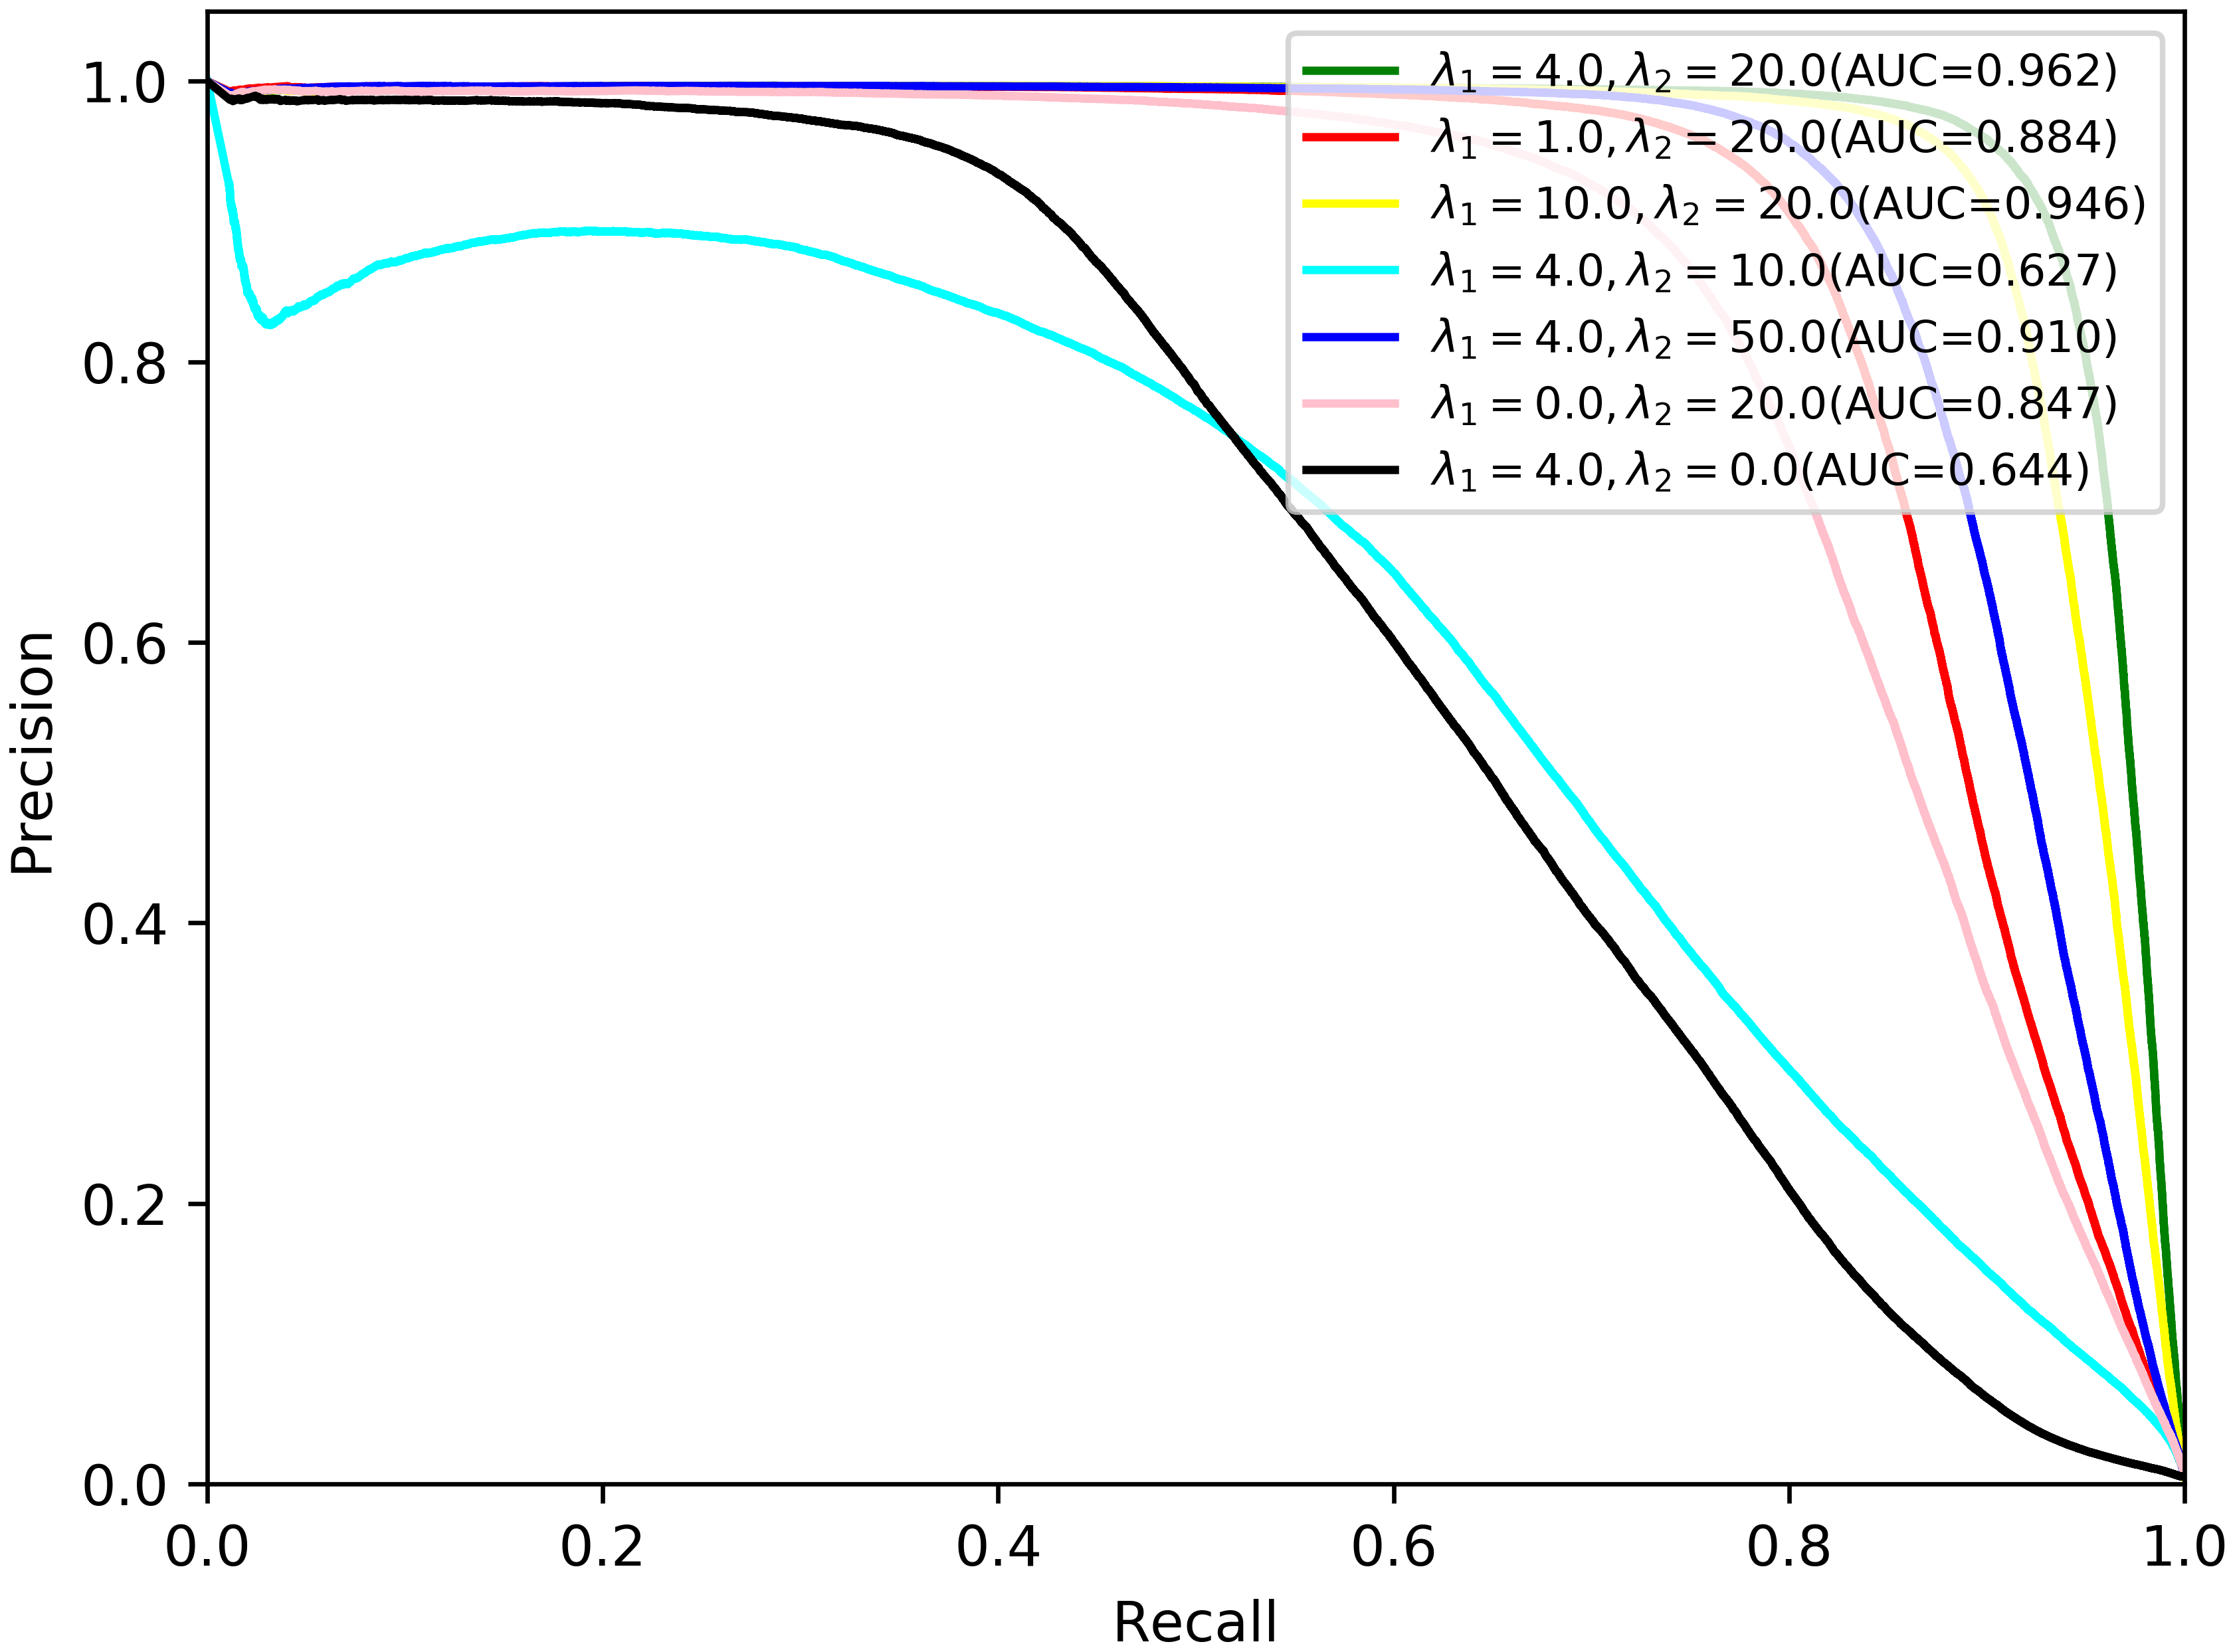
\includegraphics[width=1.0\textwidth]{figure/pr_curve_multi_skin_hyper_paras/SKIN_pr_curve.png}
	\caption{CAM、Grad-CAM-1、本文提出的模型和Grad-CAM-2在多类模拟皮肤病病变数据集的第一类异常上画出的P-R曲线及其各自曲线下的面积(AUC,见右上角图例)。} 
	\label{fig:multi_simulate_pr_curve_skin_hyper_paras}
\end{figure}

\begin{figure}[!htbp]
	\centering
	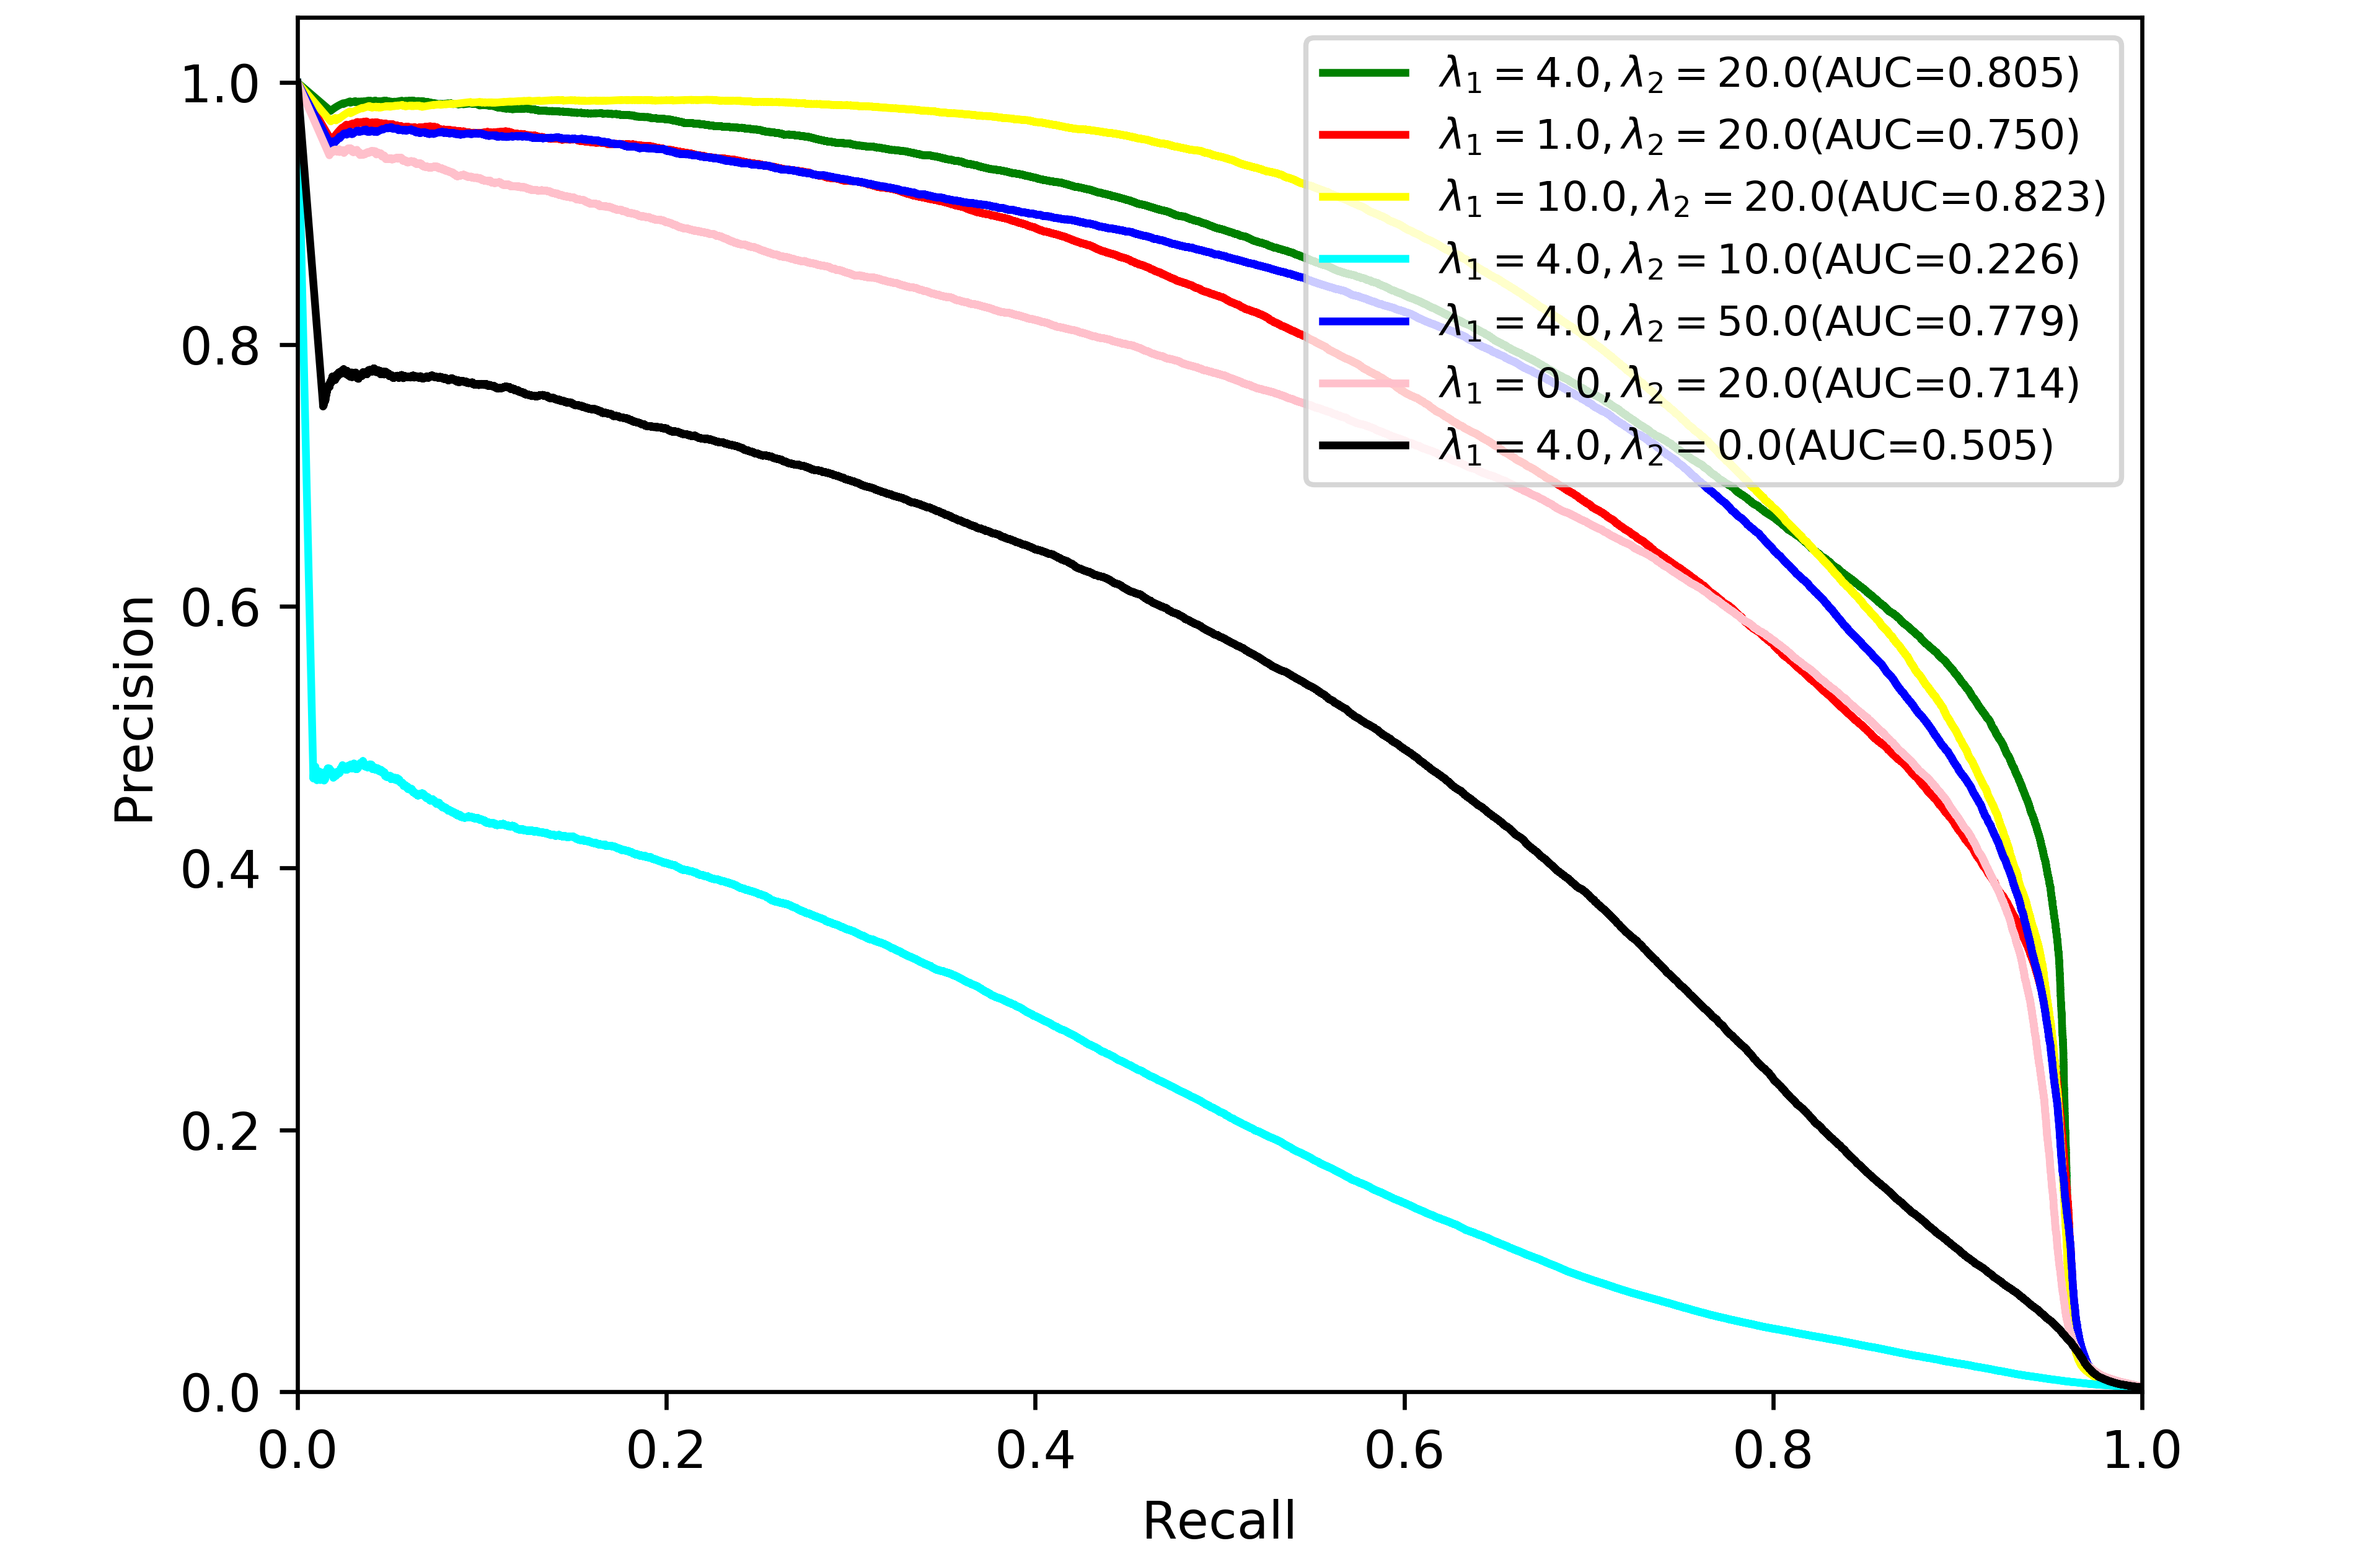
\includegraphics[width=1.0\textwidth]{figure/pr_curve_multi_skin_hyper_paras/CIRCLE_pr_curve.png}
	\caption{CAM、Grad-CAM-1、本文提出的模型和Grad-CAM-2在多类模拟皮肤病病变数据集的第一类异常上画出的P-R曲线及其各自曲线下的面积(AUC,见右上角图例)。} 
	\label{fig:multi_simulate_pr_curve_circle_hyper_paras}
\end{figure}


\begin{table}[h]
	\centering
	\caption{不同超参数组合下,本文提出的模型在二类视网膜糖尿病病变数据集上计算得到的AUC分数列表。}		
	\label{tab:simulated_skin_diff_parameters}
	\resizebox{1.0\textwidth}{!}{
		\begin{tabular}{c|c|c|c|c|c|c|c}
			\toprule[2pt]
			& $\lambda_{1}=0.8,\lambda_{2}=10$ & $\lambda_{1}=4, \lambda_{2}=10$& $\lambda_{1}=0.1, \lambda_{2}=10$&
			
			$\lambda_{1}=0.8,\lambda_{2}=20$ & $\lambda_{1}=0.8,\lambda_{2}=50$ &
			$\lambda_{1}=0,\lambda_{2}=10$ &
			$\lambda_{1}=0.8, \lambda_{2}=0$\\
			\midrule[2pt]
			第一类异常	& $0.250$ &	$0.421 $ & $0.433$ & $0.056$ & $0.085$& $0.012$ &	 \\\hline
			
			第二类异常	& $$ &	$0.421 $ & $0.433$ & $0.056$ & $0.085$& $0.012$ &	 \\\hline
			
			第三类异常	& $\textbf{0.481}$ &	$0.421 $ & $0.433$ & $0.056$ & $0.085$& $0.012$ &	 \\\hline
			
			Average AUC	& $\textbf{0.481}$ &	$0.421 $ & $0.433$ & $0.056$ & $0.085$& $0.012$ &	 \\
			\bottomrule[2pt]
		\end{tabular}
	}
\end{table}
%\section{对判别器模型结构的探究}

\section{本章小结}
本章主要将本文提出的方法由二类问题推广到多类问题,在此过程中,本文对原始二类模型进行了相关改进,比如,将二类交叉熵损失函数替换成多类交叉熵损失函数、将所有异常类看成判别器的假图像输入端等,以最小的代价实现二类问题到多类问题的扩展,并在多类模拟皮肤病病变数据集上进行了相关实验评估,与CAM和Grad-CAM相比,分别从定性分析(热图)和定量分析(P-R曲线及其AUC)两个角度直接说明本文提出的模型能够更准确地定位到生物标记物的位置,具有更加优异的性能。除此之外,本文还分别从额外训练的CNN分类器的角度和判别器的角度再次证明了上述结论。最后,为了说明本文提出的方法的超参数鲁棒性,本文还对不同超参数$\lambda_{1}$和$\lambda_{2}$组合进行了测试。到此,本文所有实验内容叙述完毕。在接下来一章中,我们将对本文工作进行总结,并对将来的研究方向进行展望。

